\section{Рабочий проект}

\subsection{Классы, используемые при разработке приложения}

\renewcommand{\arraystretch}{0.8}
\begin{xltabular}{\textwidth}{|X|p{2.5cm}|>{\setlength{\baselineskip}{0.7\baselineskip}}p{4.85cm}|>{\setlength{\baselineskip}{0.7\baselineskip}}p{4.85cm}|}
	\caption{Описание классов, используемых в приложении\label{class:table}}\\
	\hline \centrow \setlength{\baselineskip}{0.7\baselineskip} Название класса & \centrow \setlength{\baselineskip}{0.7\baselineskip} Модуль & \centrow Описание класса & \centrow Методы \\ \hline
	\endfirsthead
	\caption*{Продолжение таблицы \ref{class:table}}\\
	\hline \centrow Название класса & \centrow Модуль & \centrow Описание класса & \centrow Методы \\ \hline
	\endhead
	
	Audio- Processor & audio\_ processor.py & Основной класс для обработки аудио, реализует эффекты и управление аудиопотоком & 
	\begin{itemize}[leftmargin=*,noitemsep,topsep=0pt]
		\item \_\_init\_\_ - инициализация процессора
		\item load\_audio - загрузка аудиофайла
		\item apply\_all\_effects - применение всех эффектов
		\item process\_entire\_audio - обработка всего аудио
		\item apply\_eq - эквалайзер
		\item apply\_compressor - компрессор
		\item apply\_reverb - реверберация
		\item apply\_noise\_reduction - шумоподавление
	\end{itemize} \\
	\hline
	
	Compressor- Band & audio\_ processor.py & Dataclass для хранения параметров полосы компрессора & 
	\begin{itemize}[leftmargin=*,noitemsep,topsep=0pt]
		\item Хранит параметры: threshold, ratio, attack, release, gain, knee\_width
	\end{itemize} \\
	\hline
	
	Knob & gui.py & Кастомный виджет регулятора в виде крутящейся ручки & 
	\begin{itemize}[leftmargin=*,noitemsep,topsep=0pt]
		\item \_\_init\_\_ - инициализация
		\item \_draw\_knob - отрисовка
		\item \_on\_drag - обработка вращения
		\item \_on\_scroll - обработка колесика мыши
	\end{itemize} \\
	\hline
	
	AudioApp & gui.py & Главный класс приложения, реализует графический интерфейс & 
	\begin{itemize}[leftmargin=*,noitemsep,topsep=0pt]
		\item \_\_init\_\_ - инициализация
		\item \_create\_main\_interface - создание интерфейса
		\item load\_audio - загрузка файла
		\item \_safe\_start\_playback - воспроизведение
		\item stop\_playback - остановка
		\item save\_audio - сохранение
		\item update\_gui - обновление интерфейса
	\end{itemize} \\
	\hline
	
\end{xltabular}
\renewcommand{\arraystretch}{1.0}

\subsection{Описание элементов интерфейса пользователя}

На рисунке \ref{InterProg:image} интерфейс программы при запуске.

\begin{enumerate}
	\item Окно отображения графика формы волны.
	\item Окно отображения графика АЧХ.
	\item Кнопка загрузки аудиофайла (активно).
	\item Кнопка воспроизведения аудио (активно).
	\item Кнопка остановки аудио (неактивна).
	\item Кнопка сохранения аудио (неактивно).
	\item Кнопка шумоподавления (неактивно).
	\item Knob регулировки уровня шумоподавления.
	\item Отображение процентов воздействия шумподавления на аудио.
	\item Слайдер отслеживания и управление временем воспроизведения.
	\item Время аудио нынешнее/полное.
	\item Активная вкладка открытого окна эквалайзера.
	\item Неактивная вкладка закрытого окна компрессора.
	\item Неактивная вкладка закрытого окна реверберации.
	\item Чекбокс включения эквалайзера.
	\item Слайдер регулировки уровня частоты 50 Гц с подписанным снизу параметром настройки.
	\item Слайдер регулировки уровня частоты 150 Гц с подписанным снизу параметром настройки.
	\item Слайдер регулировки уровня частоты 250 Гц с подписанным снизу параметром настройки.
	\item Слайдер регулировки уровня частоты 500 Гц с подписанным снизу параметром настройки.
	\item Слайдер регулировки уровня частоты 1 кГц с подписанным снизу параметром настройки.
	\item Слайдер регулировки уровня частоты 3 кГц с подписанным снизу параметром настройки.
	\item Слайдер регулировки уровня частоты 7 кГц с подписанным снизу параметром настройки.
	\item Слайдер регулировки уровня частоты 15 кГц с подписанным снизу параметром настройки.
\end{enumerate}

\begin{figure}[ht]
	\center{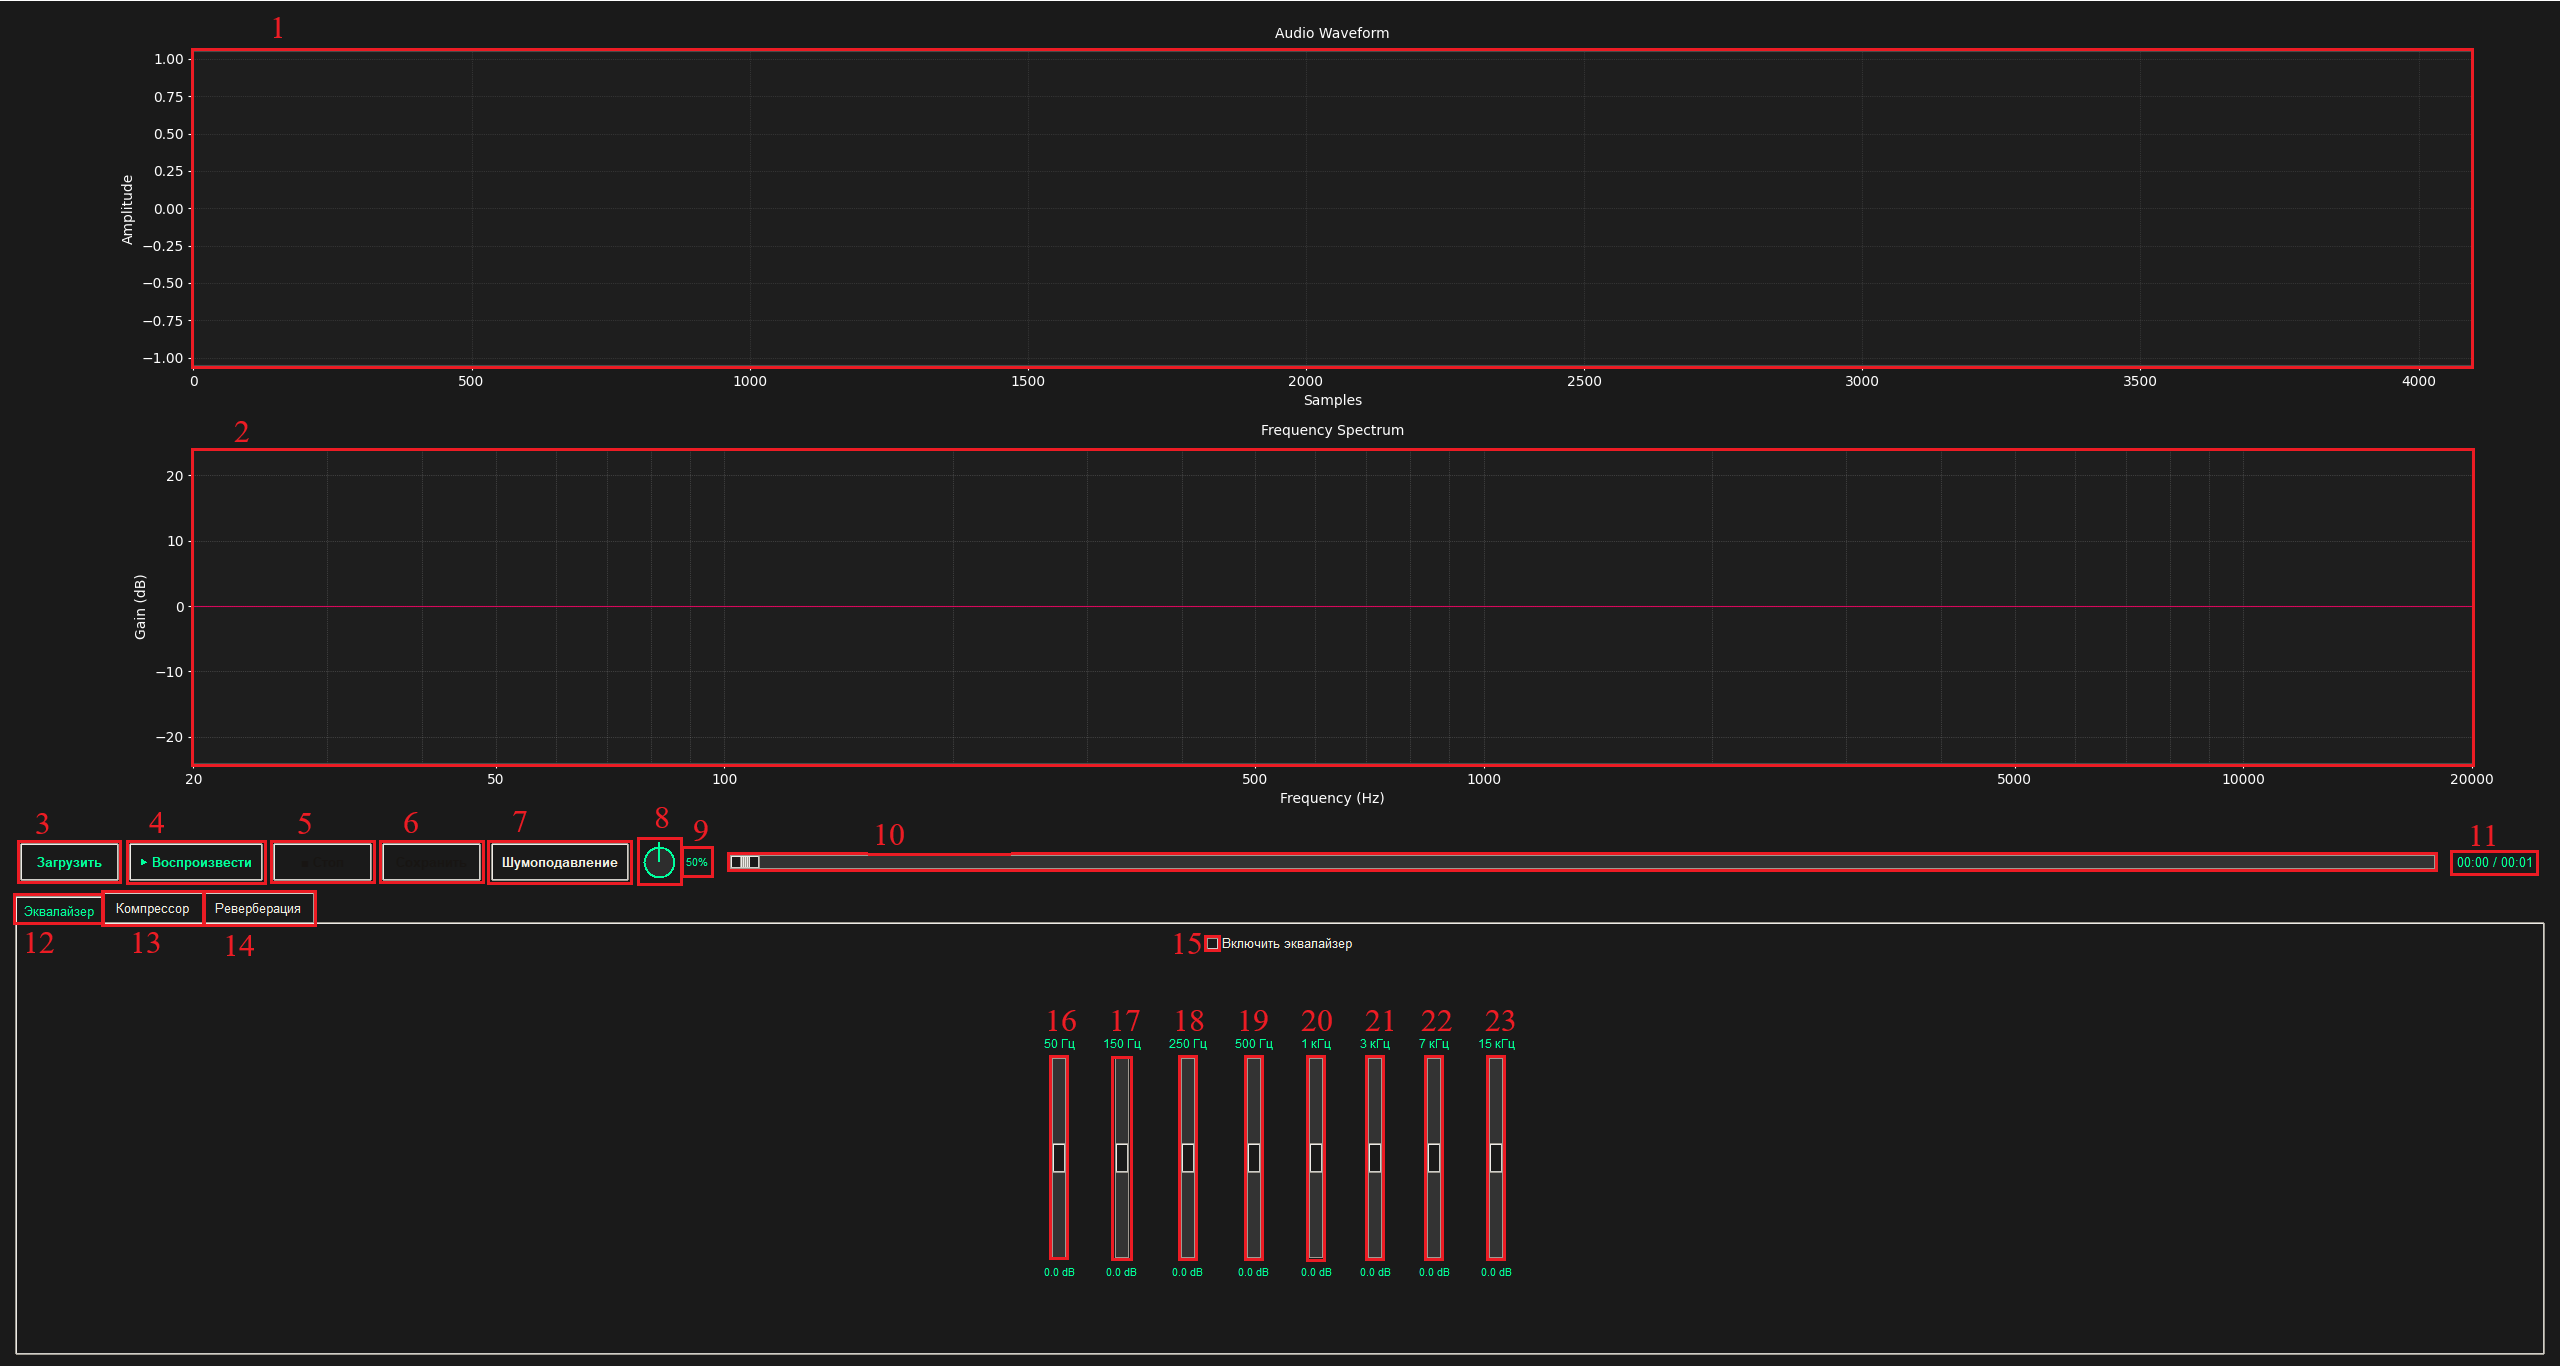
\includegraphics[width=1\linewidth]{InterProg}}
	\caption{Интерфейс приложения при запуске.}
	\label{InterProg:image}
\end{figure}

На рисунке \ref{WindLoad:image} окно загрузки аудиофайла.

\begin{figure}[ht]
	\center{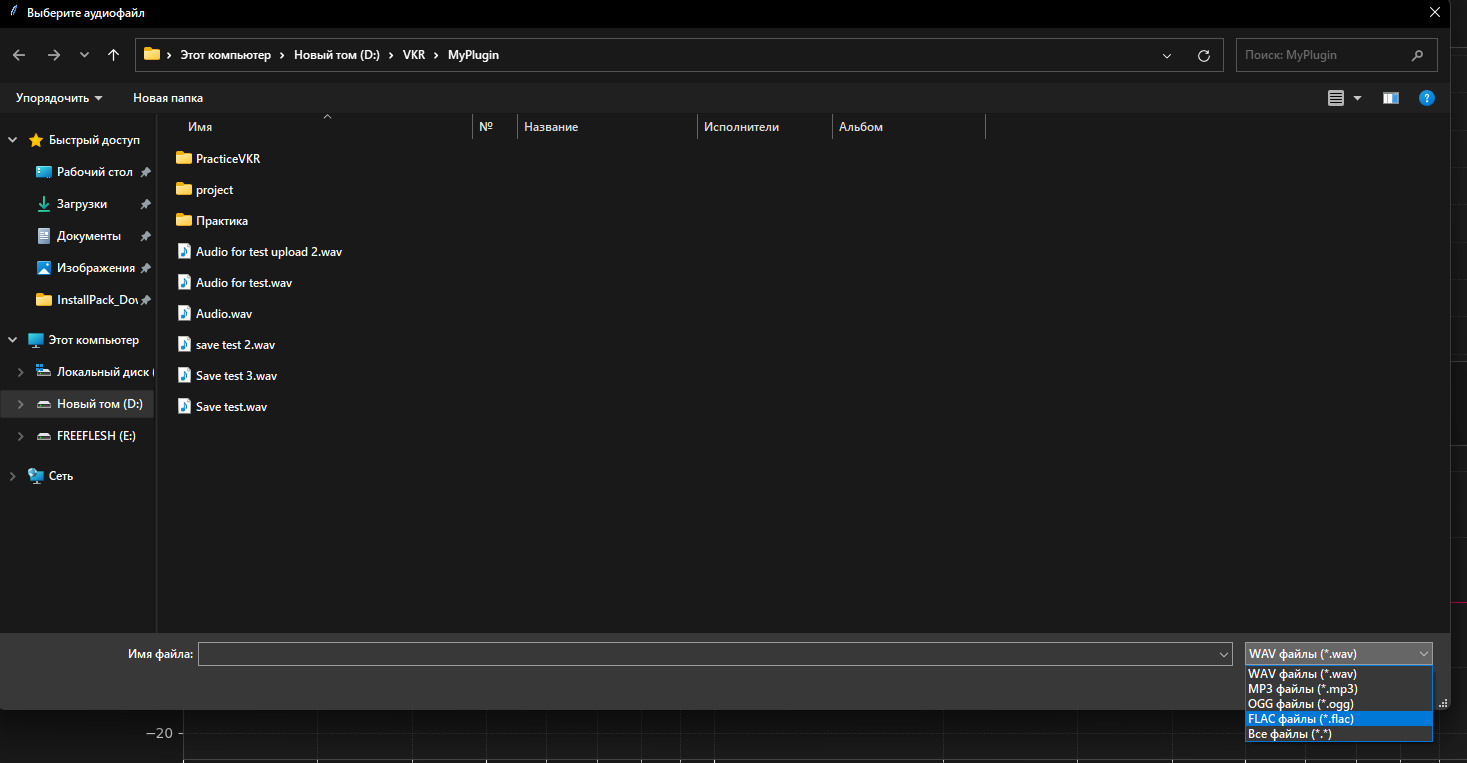
\includegraphics[width=1\linewidth]{WindLoad}}
	\caption{Окно загрузки аудиофайла.}
	\label{WindLoad:image}
\end{figure}

На рисунке \ref{CompWind:image} интерфейс вкладки компрессора.

\begin{enumerate}
	\item Кнопка воспроизведения аудио (неактивно).
	\item Кнопка остановки аудио (активно).
	\item Кнопка сохранения аудио (активно).
	\item Активная кнопка шумоподавления.
	\item Окно регулировки диапазонов обработки частот.
	\item Ползунок регулировки диапазона низких частот.
	\item Ползунок регулировки диапазона высоких частот.
	\item Подпись диапазонов.
	\item Неактивный чекбокс bypass.
	\item Knob регулировки Threshold с подписью значения настройки (аналагично для всех диапазонов).
	\item Knob регулировки Ratio с подписью значения настройки (аналагично для всех диапазонов).
	\item Knob регулировки Knee с подписью значения настройки (аналагично для всех диапазонов).
	\item Knob регулировки Attack с подписью значения настройки (аналагично для всех диапазонов).
	\item Knob регулировки Release с подписью значения настройки (аналагично для всех диапазонов).	
	\item Knob регулировки Gain с подписью значения настройки (аналагично для всех диапазонов).
	\item Чекбокс активного включения компрессора.
	\item Чекбокс активного bypass.
\end{enumerate}

\begin{figure}[ht]
	\center{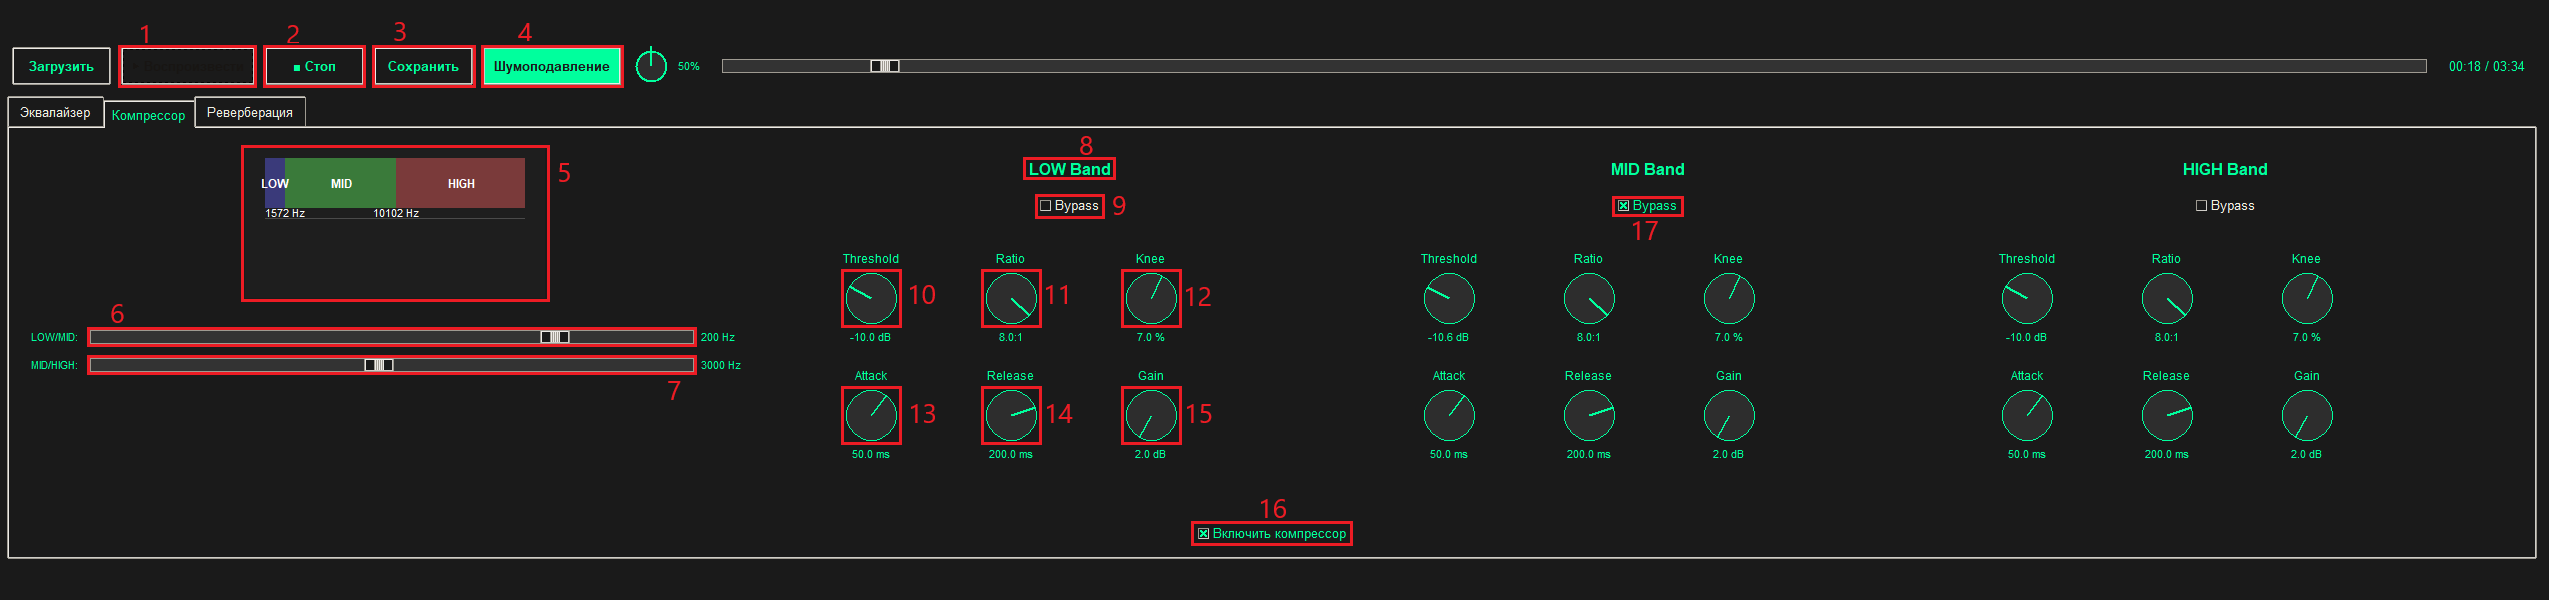
\includegraphics[width=1\linewidth]{CompWind}}
	\caption{Интерфейс вкладки компрессора.}
	\label{CompWind:image}
\end{figure}

На рисунке \ref{ReverbWind:image} интерфейс вкладки реверберации.

\begin{enumerate}
	\item Knob регулировки Wet с подписью значения настройки.
	\item Knob регулировки Dry с подписью значения настройки.
	\item Knob регулировки Size с подписью значения настройки.
	\item Knob регулировки Damping с подписью значения настройки.
	\item Knob регулировки High Cut с подписью значения настройки.
	\item Knob регулировки Low Cut с подписью значения настройки.
	\item Knob регулировки Pan с подписью значения настройки.
	\item Чекбокс активации реверберации (неактивно).
\end{enumerate}

\begin{figure}[ht]
	\center{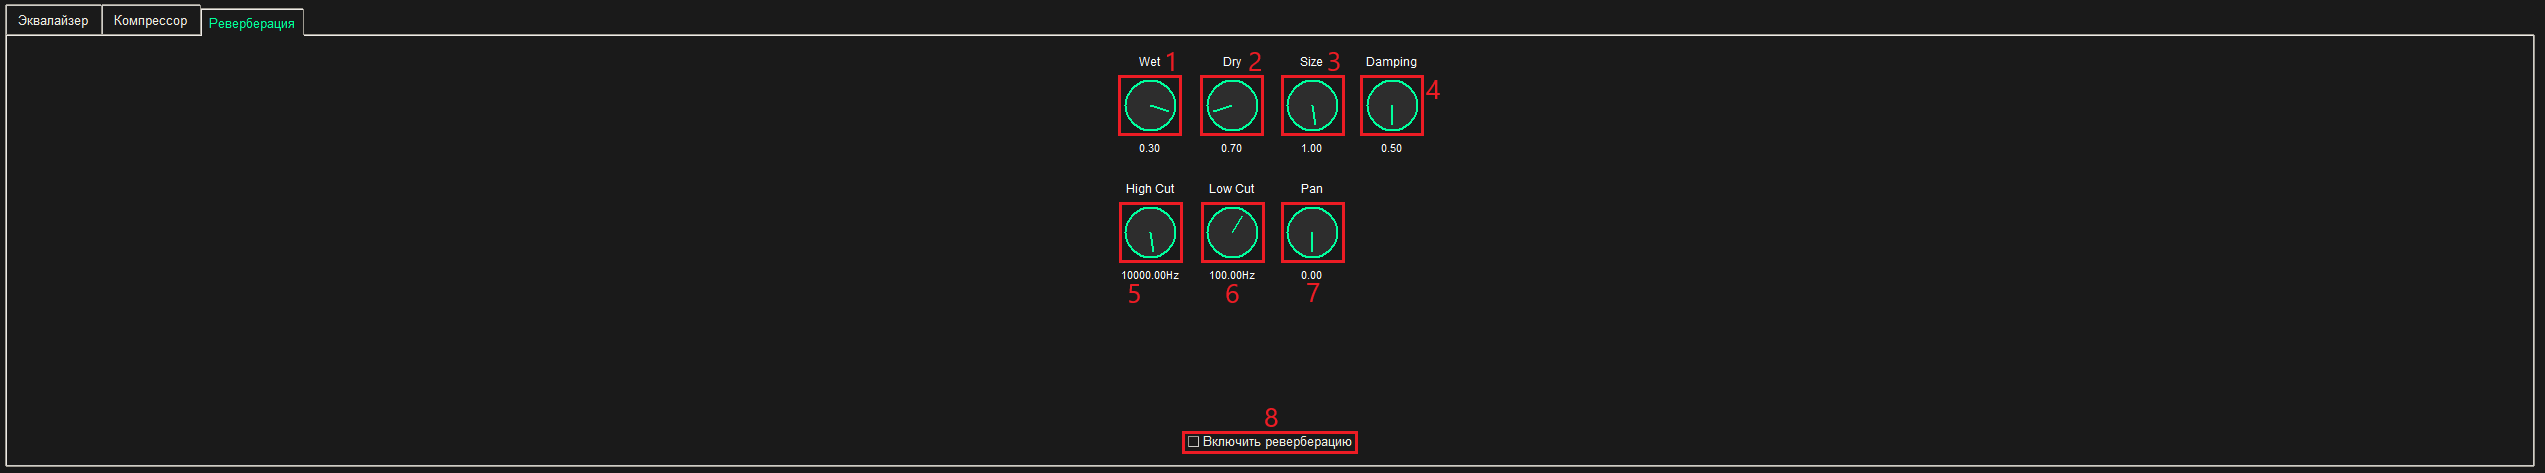
\includegraphics[width=1\linewidth]{ReverbWind}}
	\caption{Интерфейс вкладки реверберации.}
	\label{ReverbWind:image}
\end{figure}

На рисунке \ref{SaveWind:image} окно сохранения аудиофайла.

\begin{figure}[ht]
	\center{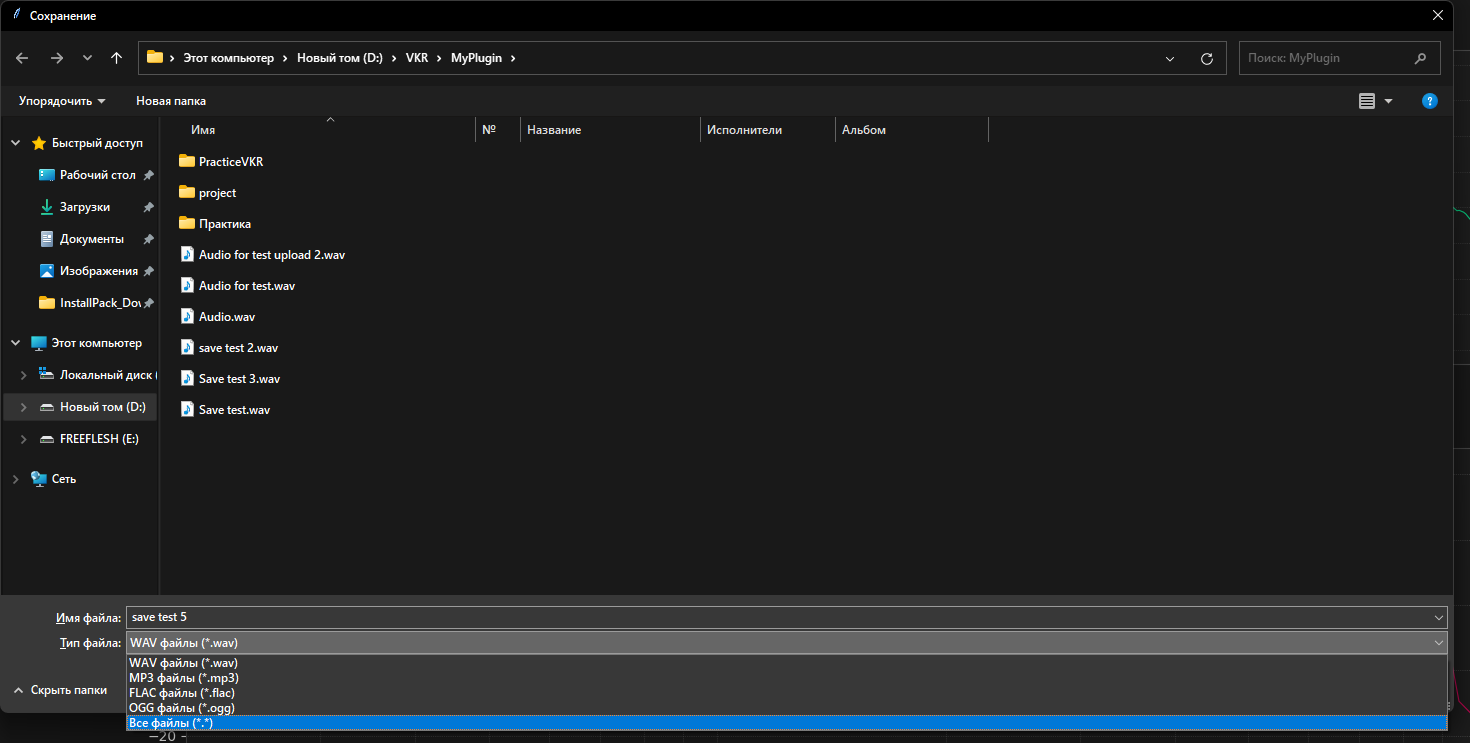
\includegraphics[width=1\linewidth]{SaveWind}}
	\caption{Окно сохранения аудиофайла.}
	\label{SaveWind:image}
\end{figure}

\subsection{Тестирование программно-информационной системы}

Тестирование аудиопроцессора — комплексный процесс, включающий проверку корректности работы всех модулей, качество обработки звука, устойчивость к ошибкам и соответствие требованиям. Для обеспечения высокого качества и надёжности программно-информационной системы необходимо провести как позитивное, так и негативное тестирование с использованием различных методов и сценариев.

\clearpage
\textbf{1) Запуск приложения}

Описание: Пользователь открывает приложение и оно запускается без ошибок и отображает рабочий интерфейс.

На рисунке \ref{Interface:image} интерфейс программы.

\begin{figure}[ht]
	\center{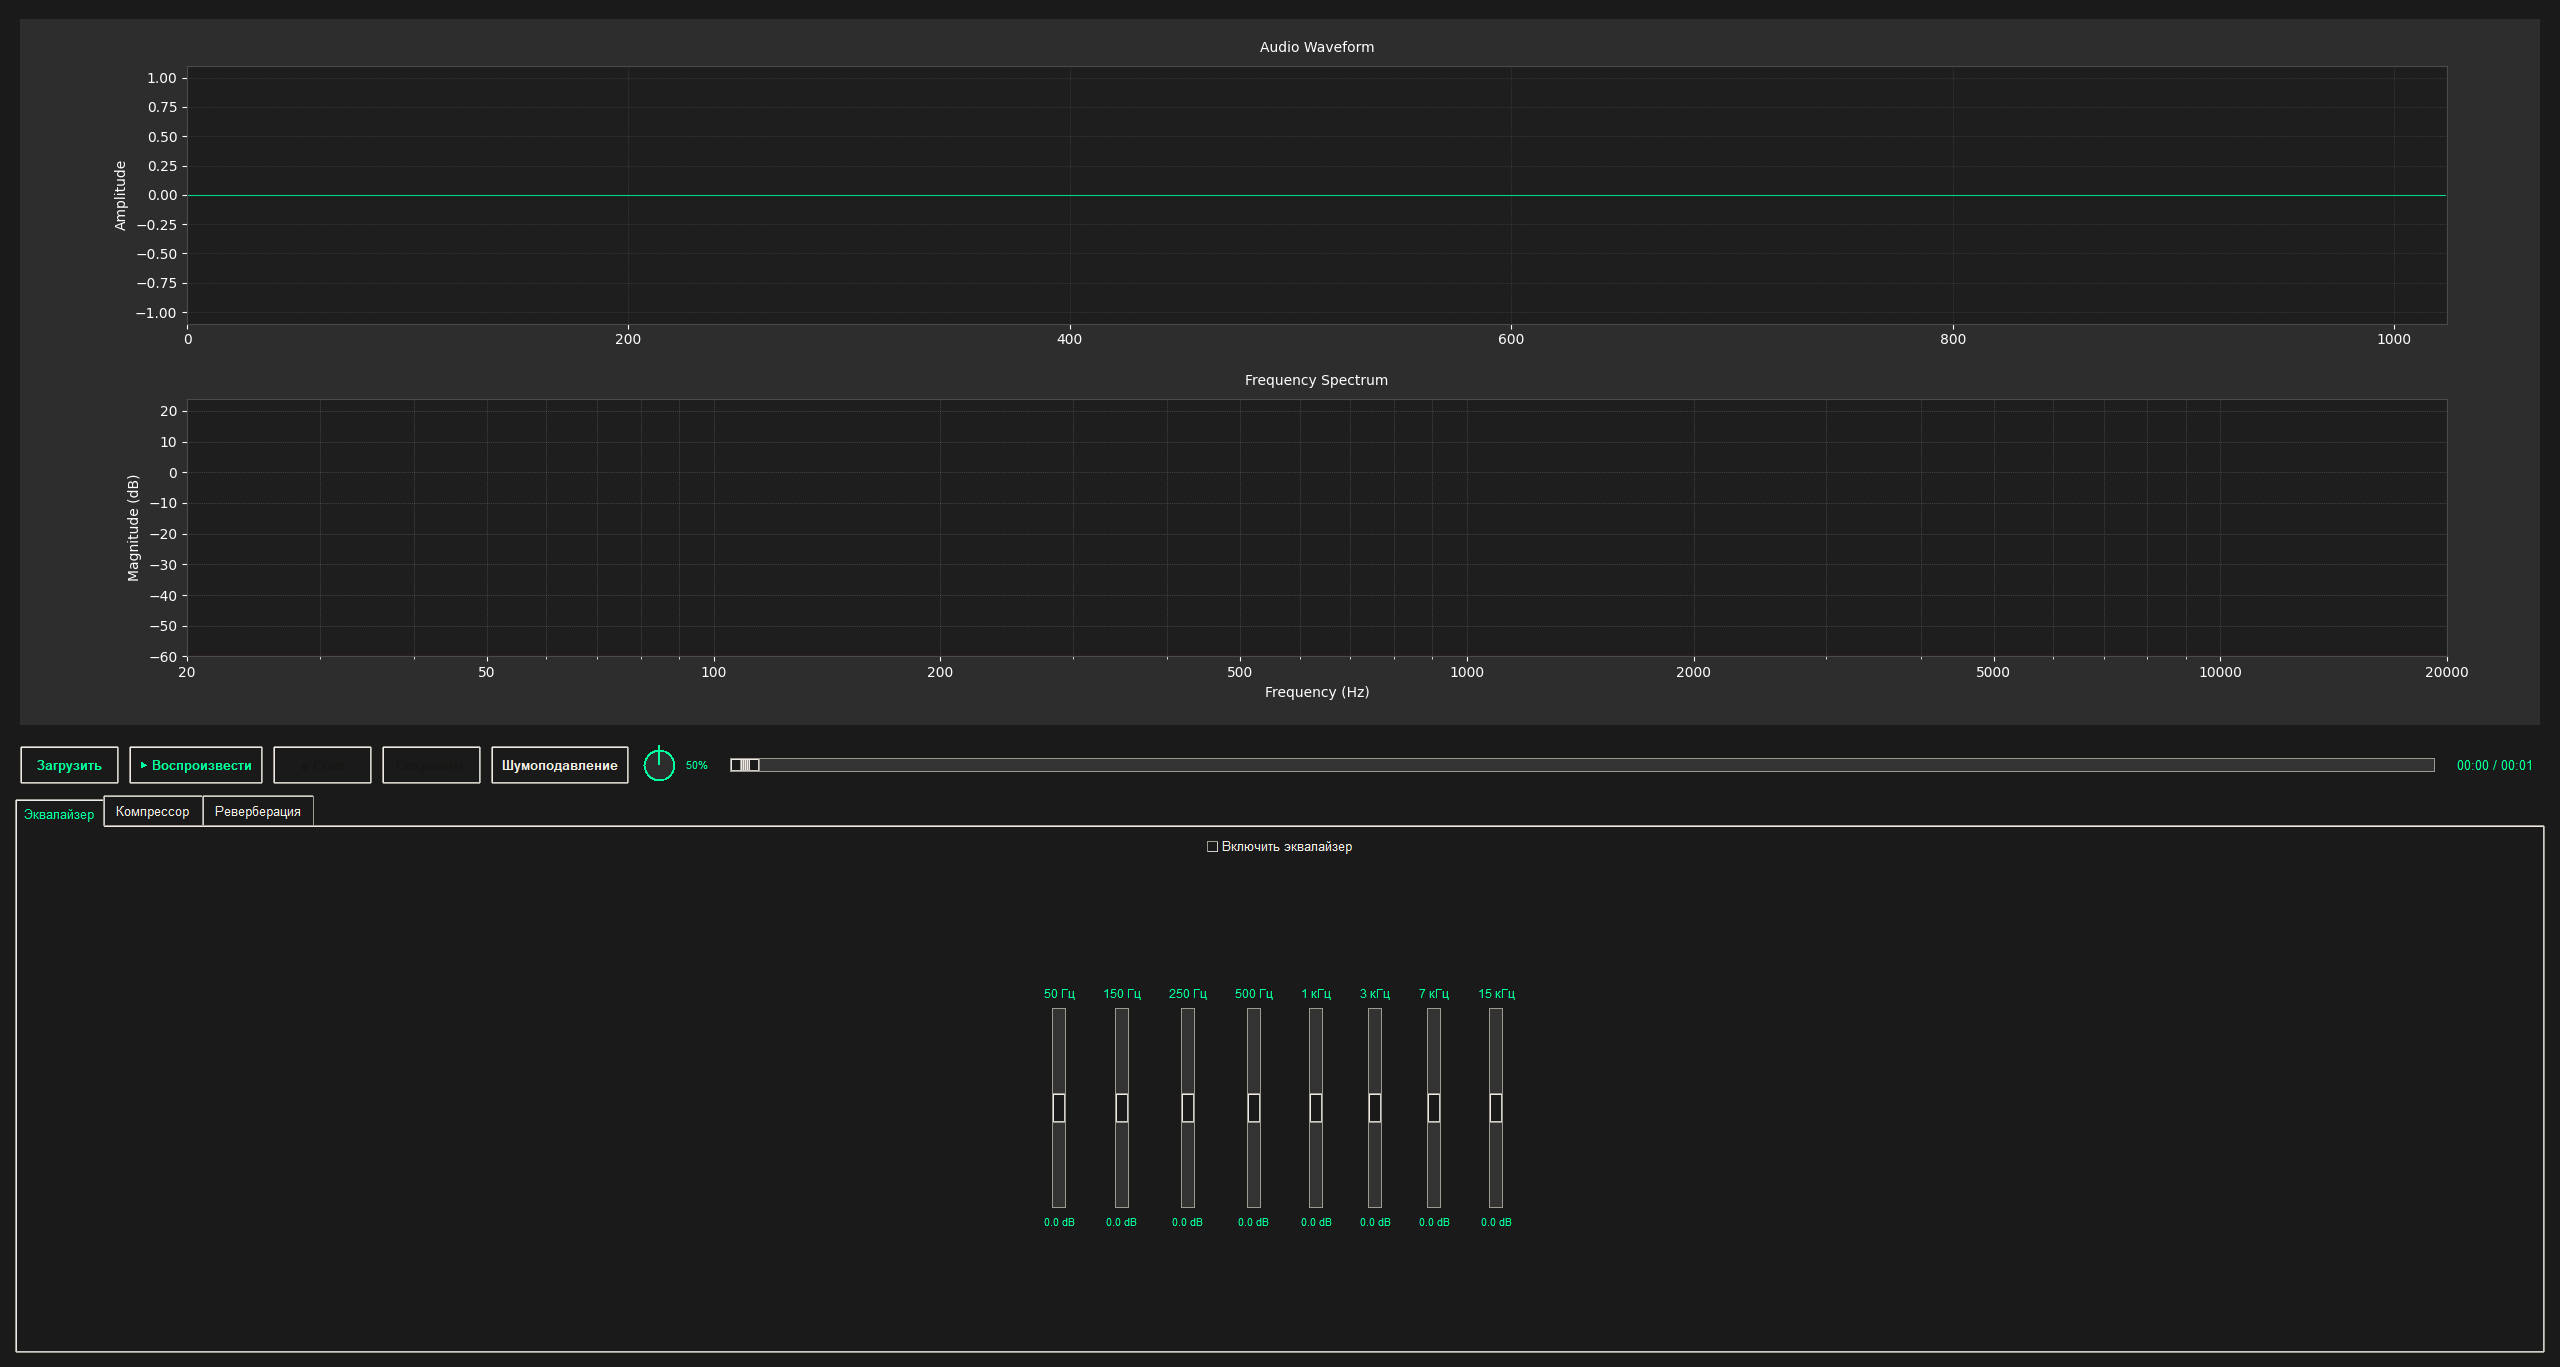
\includegraphics[width=0.8\linewidth]{Interface}}
	\caption{Интерфейс программы.}
	\label{Interface:image}
\end{figure}
\clearpage

\textbf{2) Загрузка аудиофайла}

Описание: Корректная загрузка аудиофайлов различных форматов (WAV, MP3, FLAC).

На рисунке \ref{LoadWindow:image} окно загрузки аудиофайла.

\begin{figure}[ht]
	\center{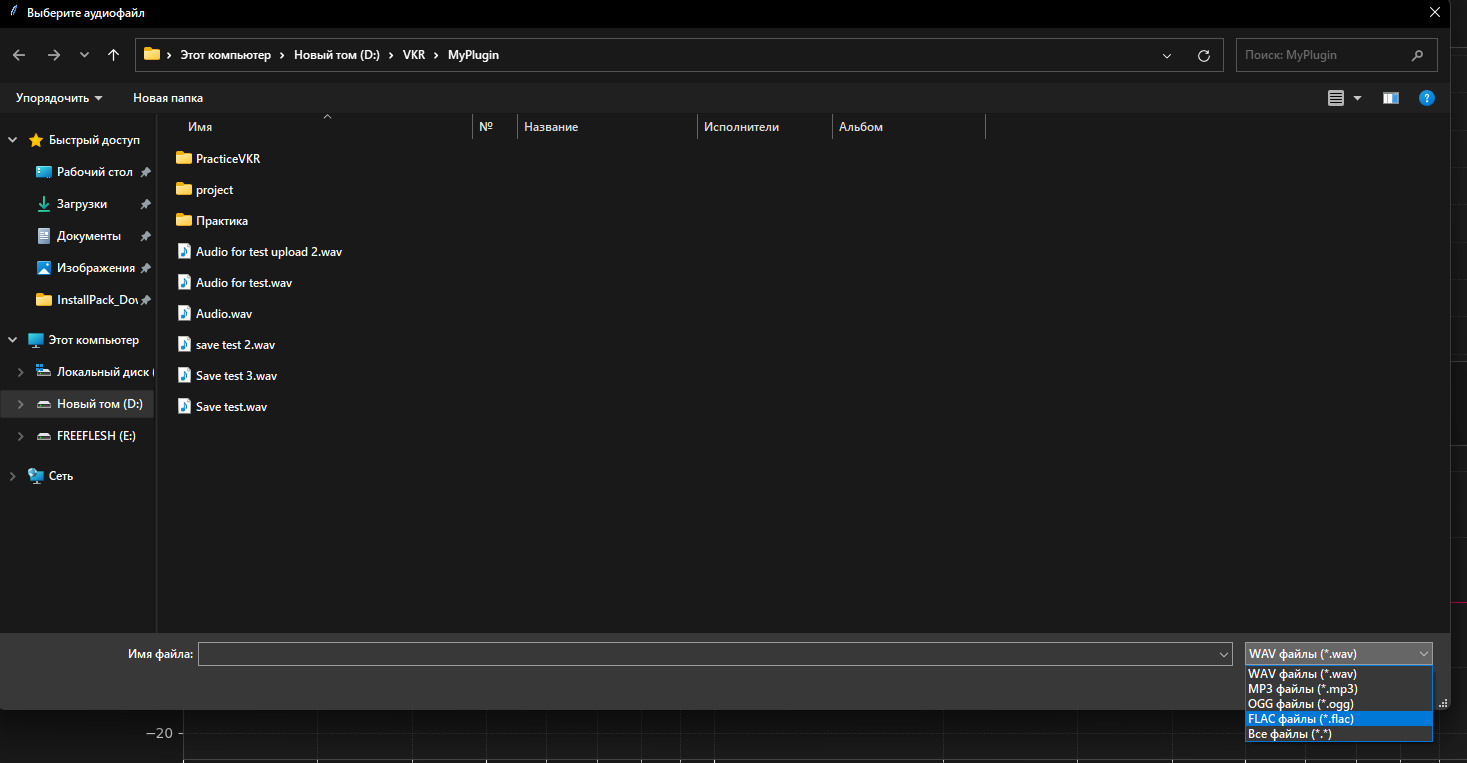
\includegraphics[width=0.8\linewidth]{LoadWindow}}
	\caption{Окно загрузки аудиофайла.}
	\label{LoadWindow:image}
\end{figure}

На рисунке \ref{InterLoad:image} интерфейс программы при успешной загрузки аудиофайла.

\begin{figure}[ht]
	\center{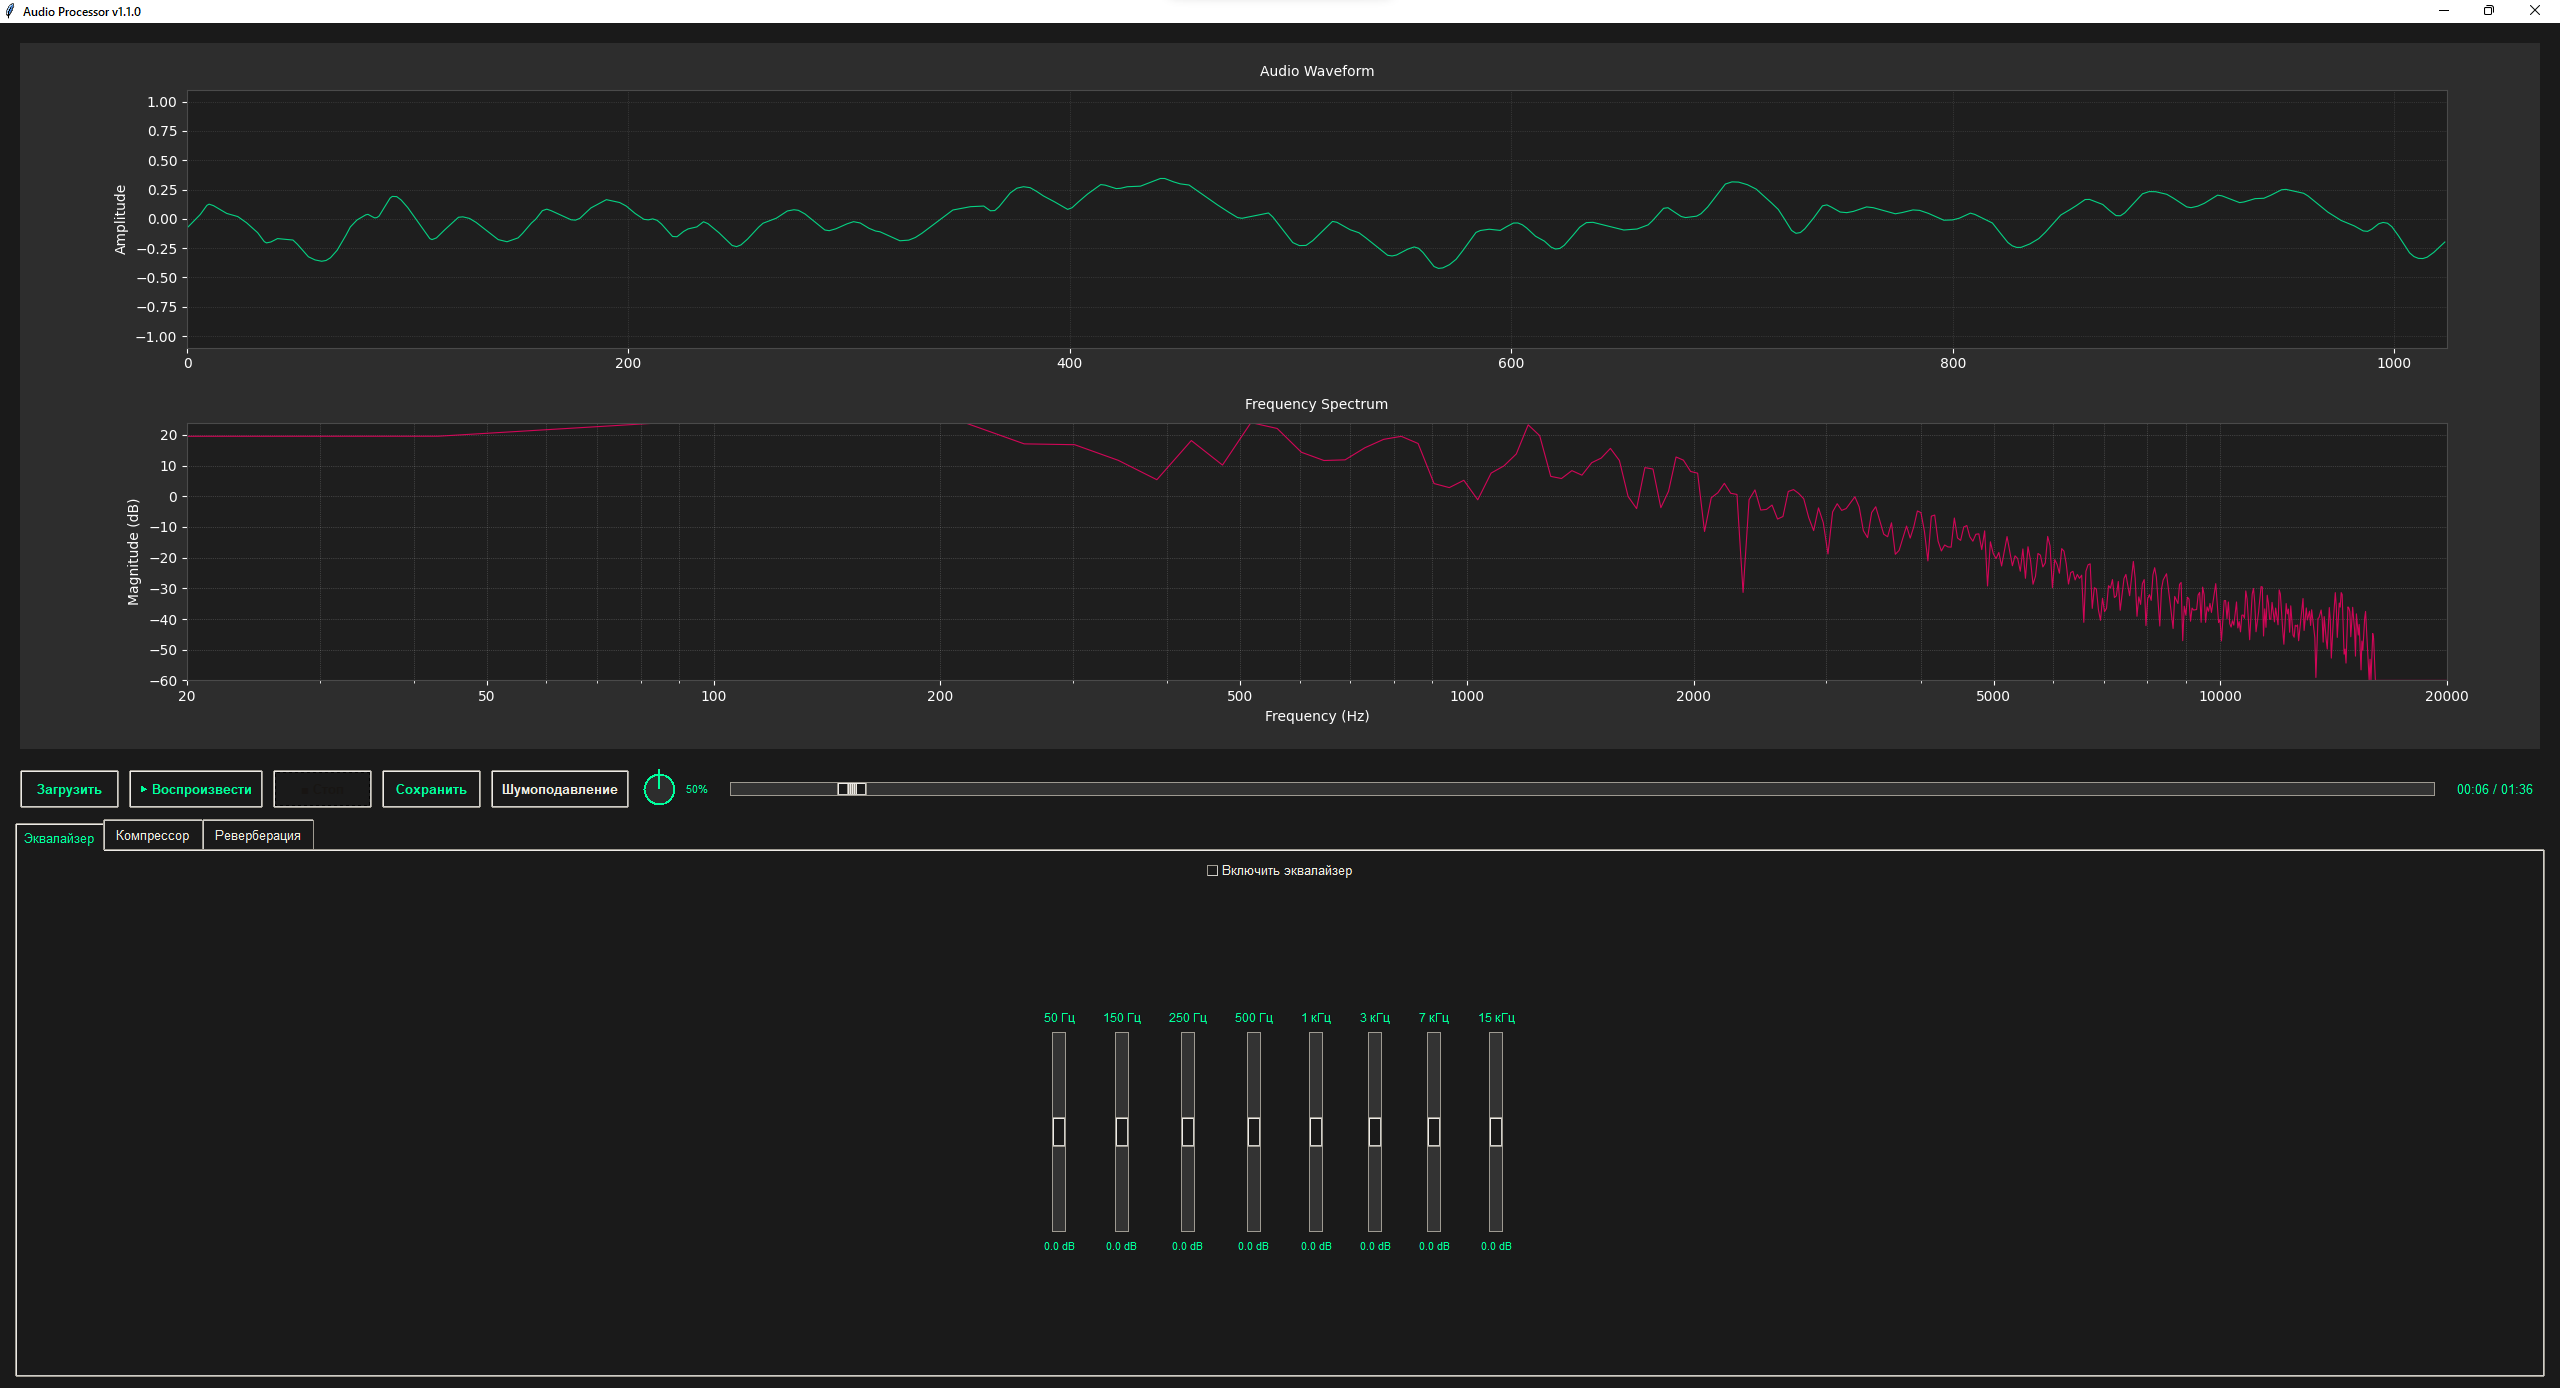
\includegraphics[width=0.8\linewidth]{InterLoad}}
	\caption{Интерфейс программы при успешной загрузки аудиофайла.}
	\label{InterLoad:image}
\end{figure}

\textbf{3) Корректное воспроизведение и остановка аудио}

Описание: При восопроизведении и остановки проигрывания аудио, соответственно, воспроизводится и останавливается. Так же перемещается ползунок метки воспроизведения в соответствии времени воспроизведения и при перемещени пользователем, аудио воспроизводится с момента, на который переместил пользователь.

На рисунке \ref{SliderTime:image} перемещение ползунка при воспроизведении.

\begin{figure}[ht]
	\center{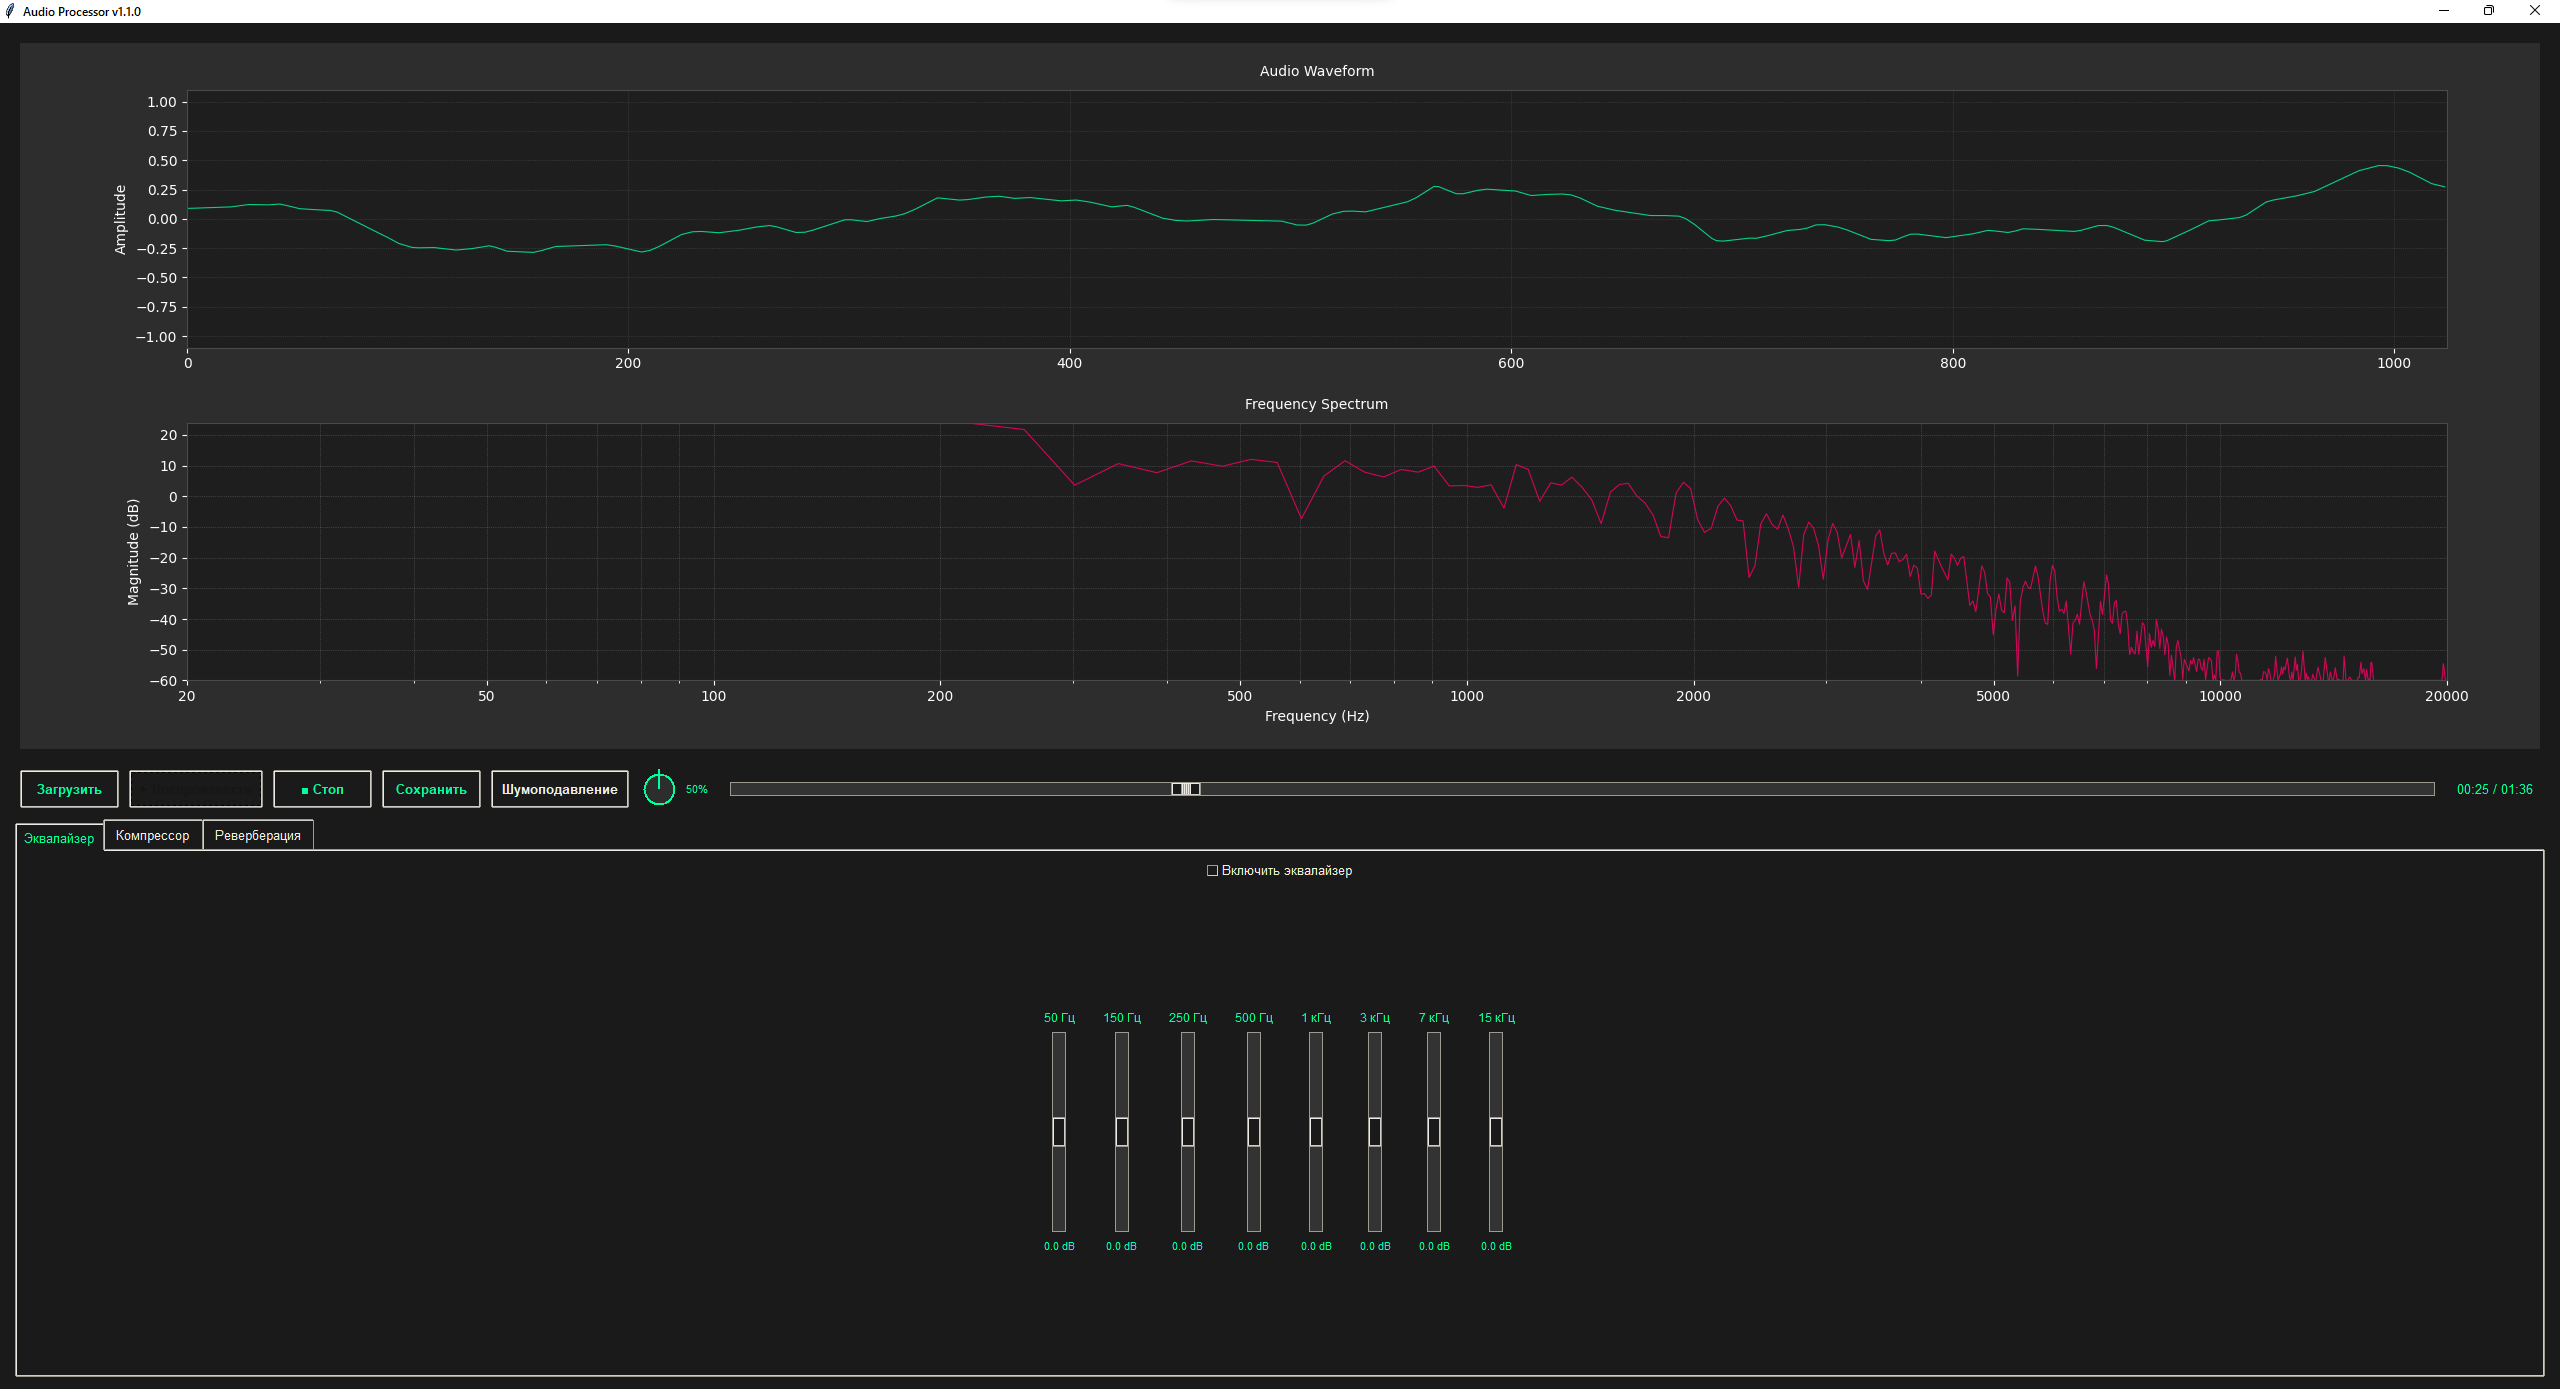
\includegraphics[width=0.8\linewidth]{SliderTime}}
	\caption{Интерфейс программы при перемещении ползунка управления воспроизведением.}
	\label{SliderTime:image}
\end{figure}
\clearpage

\textbf{4) Обработка аудиосигнала в реальном времени}

Описание: При восопроизведении аудиофайла графики формы волны и АЧХ отображают данные аудио в реальном времени.

На рисунке \ref{Graph:image} отображение графиков формы волны и АЧХ в реальном времени.

\begin{figure}[ht]
	\center{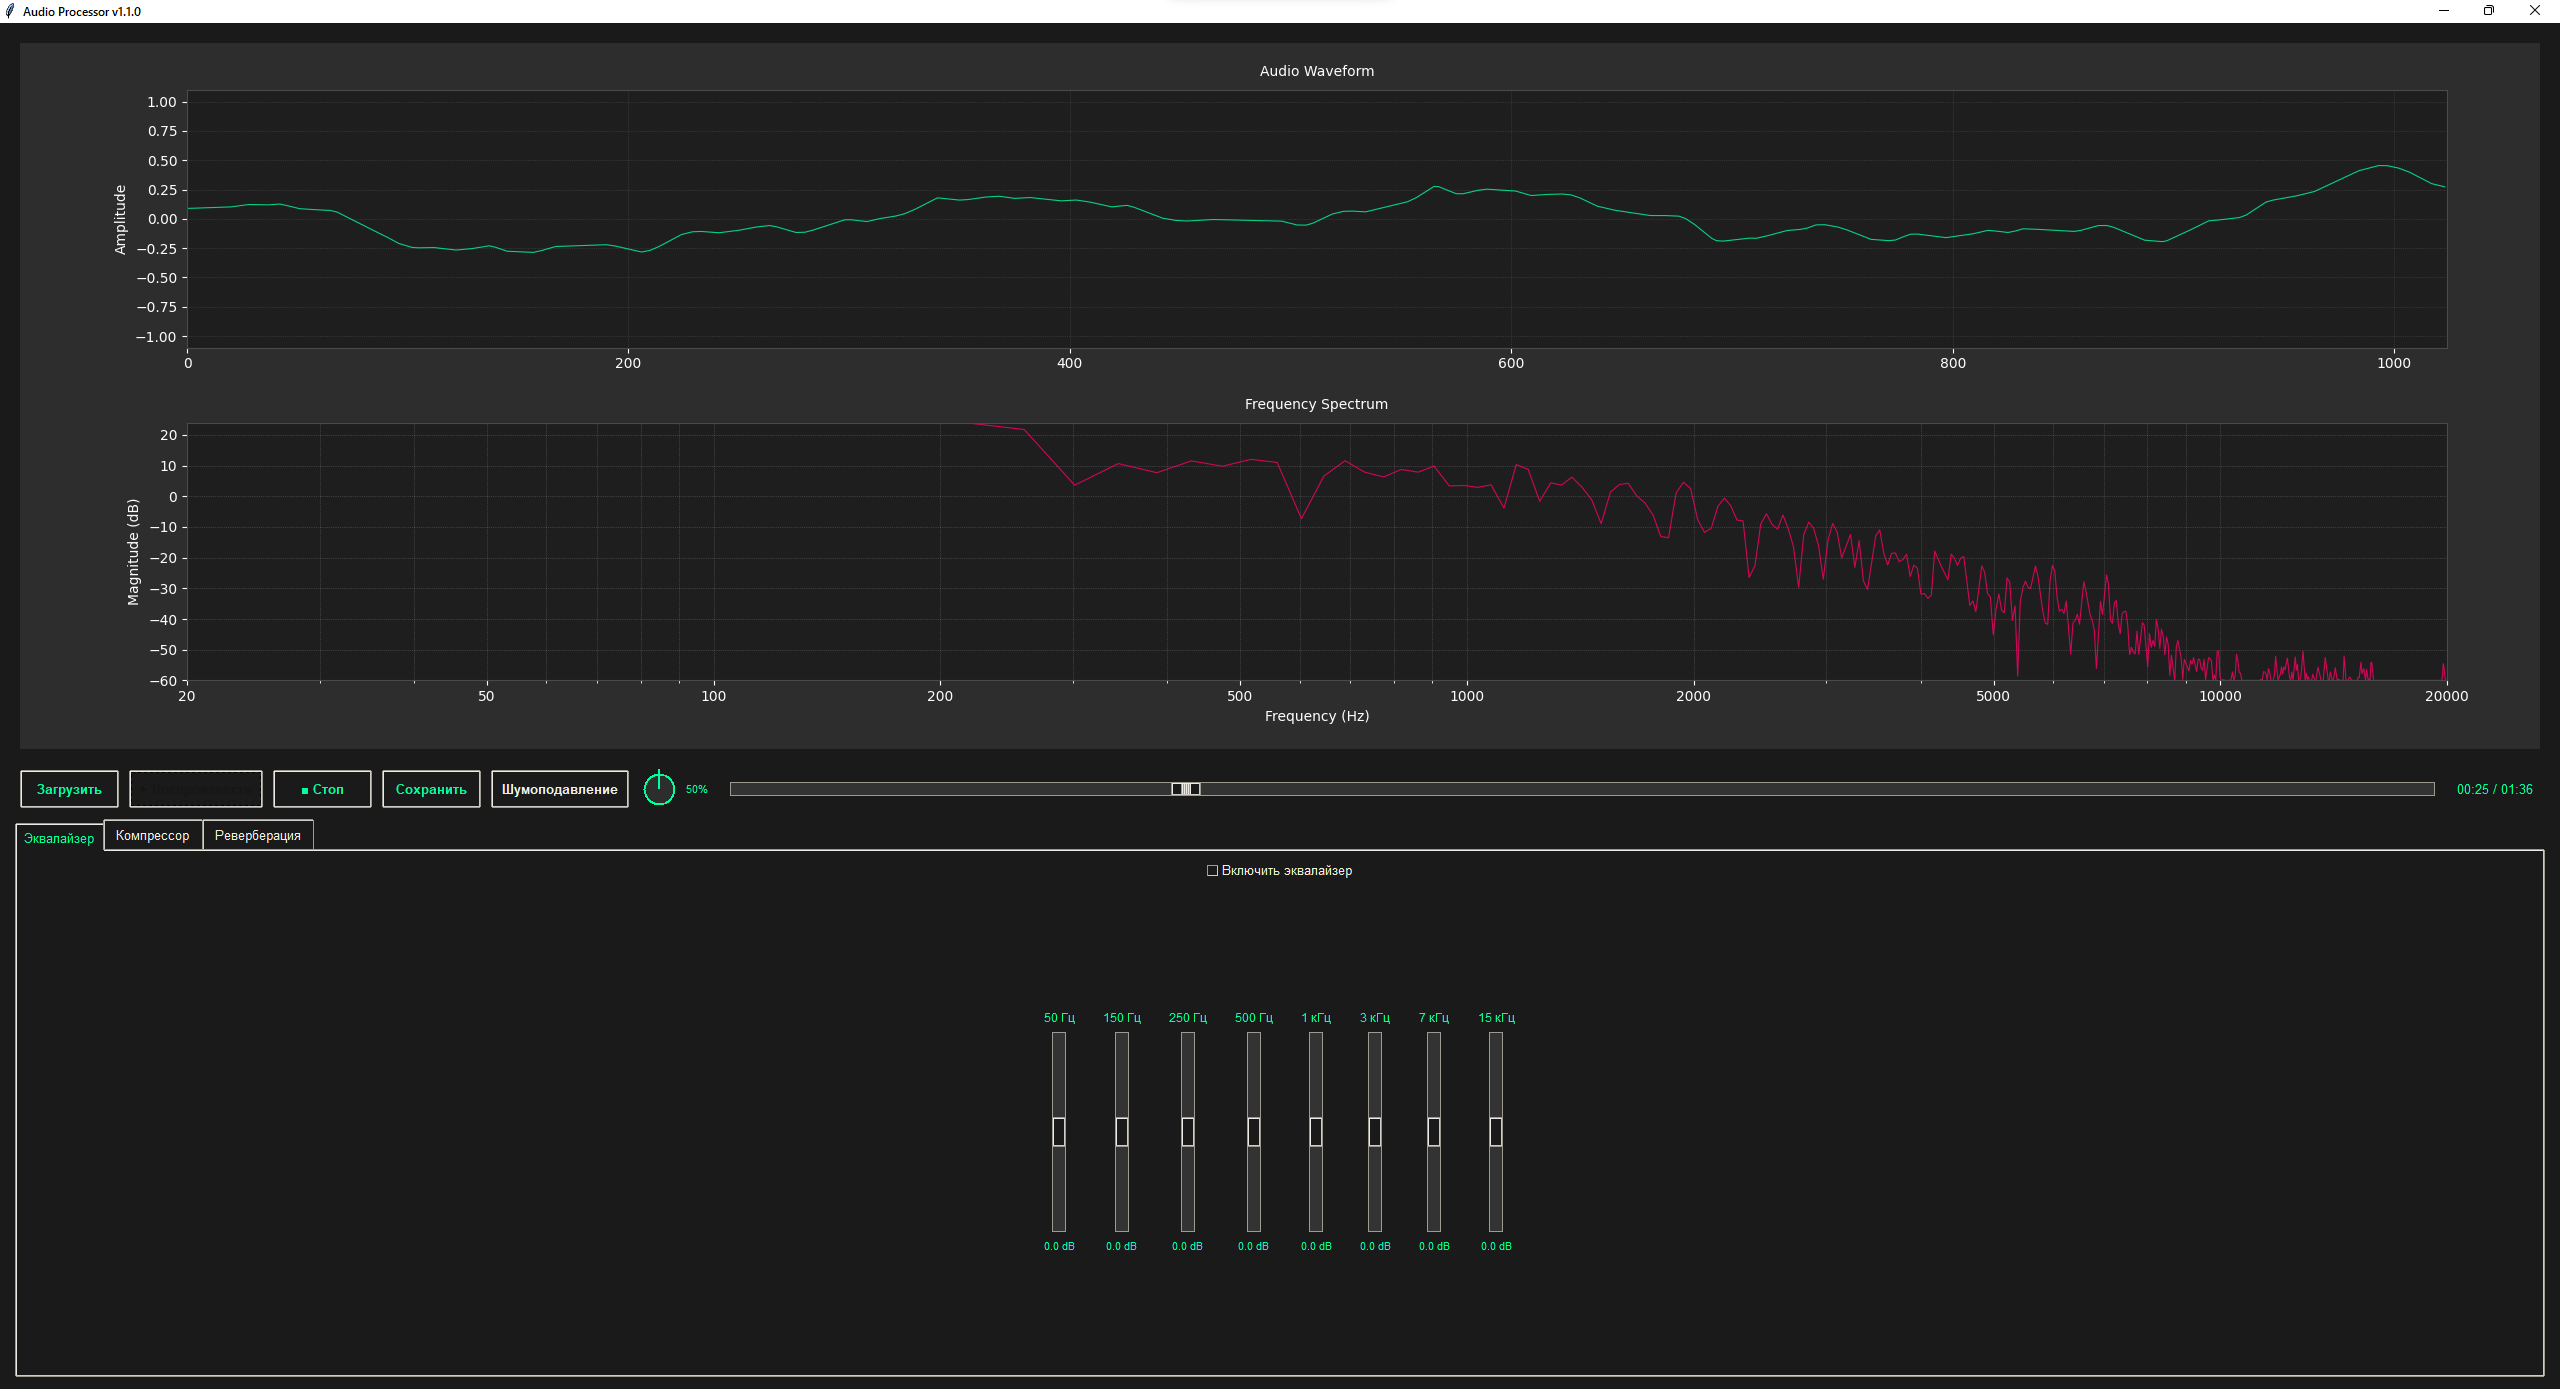
\includegraphics[width=0.8\linewidth]{Graph}}
	\caption{Отображение графиков.}
	\label{Graph:image}
\end{figure}
\clearpage

\textbf{5) Изменение параметров эквалайзера}

Описание: При изменении параметров эквалайзера, регулировки ползунков, все изменения применяются сразу, без задержек и прерываний. Так же изменяются графики формы волны и АЧХ.

На рисунке \ref{EQParam:image} изменение параметров эквалайзера.

\begin{figure}[ht]
	\center{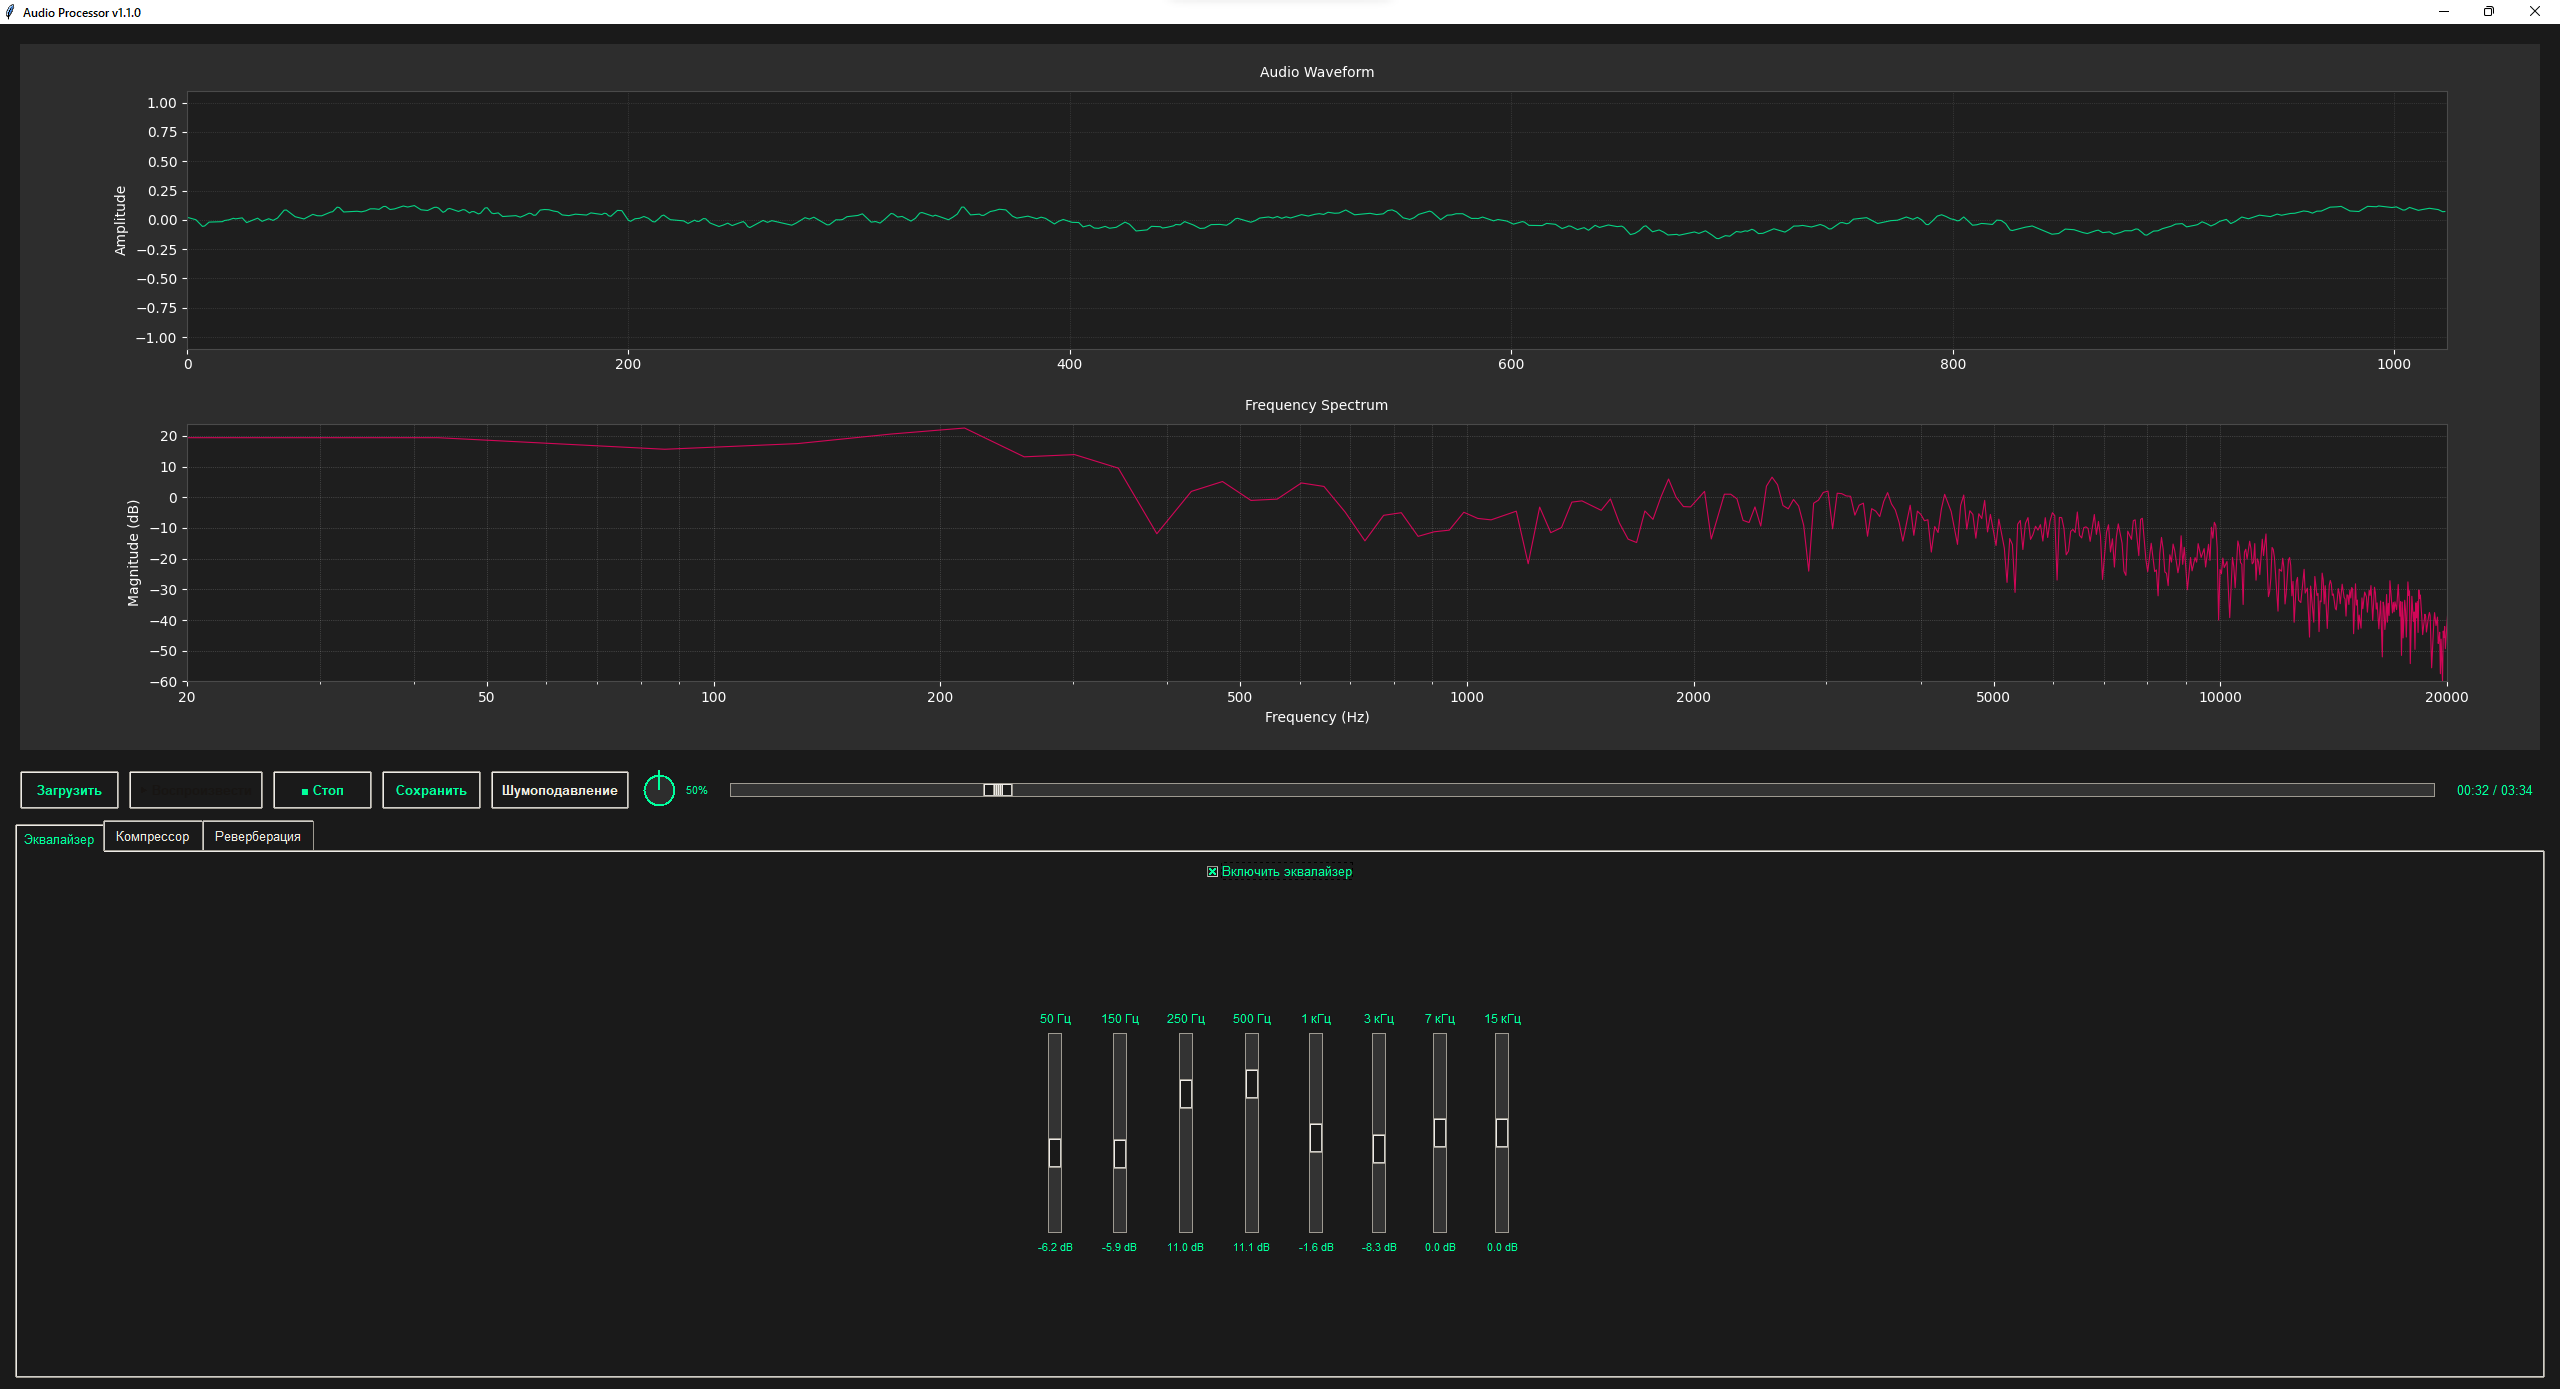
\includegraphics[width=0.8\linewidth]{EQParam}}
	\caption{Изменение параметров эквалайзера.}
	\label{EQParam:image}
\end{figure}

\clearpage
\textbf{6) Изменение параметров компрессора}

Описание: При изменении параметров компрессора, регулировки knob, все изменения применяются сразу, без задержек и прерываний. При включении/выключении функции bypass она работает корректно, то есть пропускает исходный сигнал выбранной зоны. Ползунки выбрания зон работают исправно и частотные диапазоны выделяются корректно. Так же изменяются графики формы волны и АЧХ.

На рисунке \ref{CompParam:image} изменение параметров компрессора.

\begin{figure}[ht]
	\center{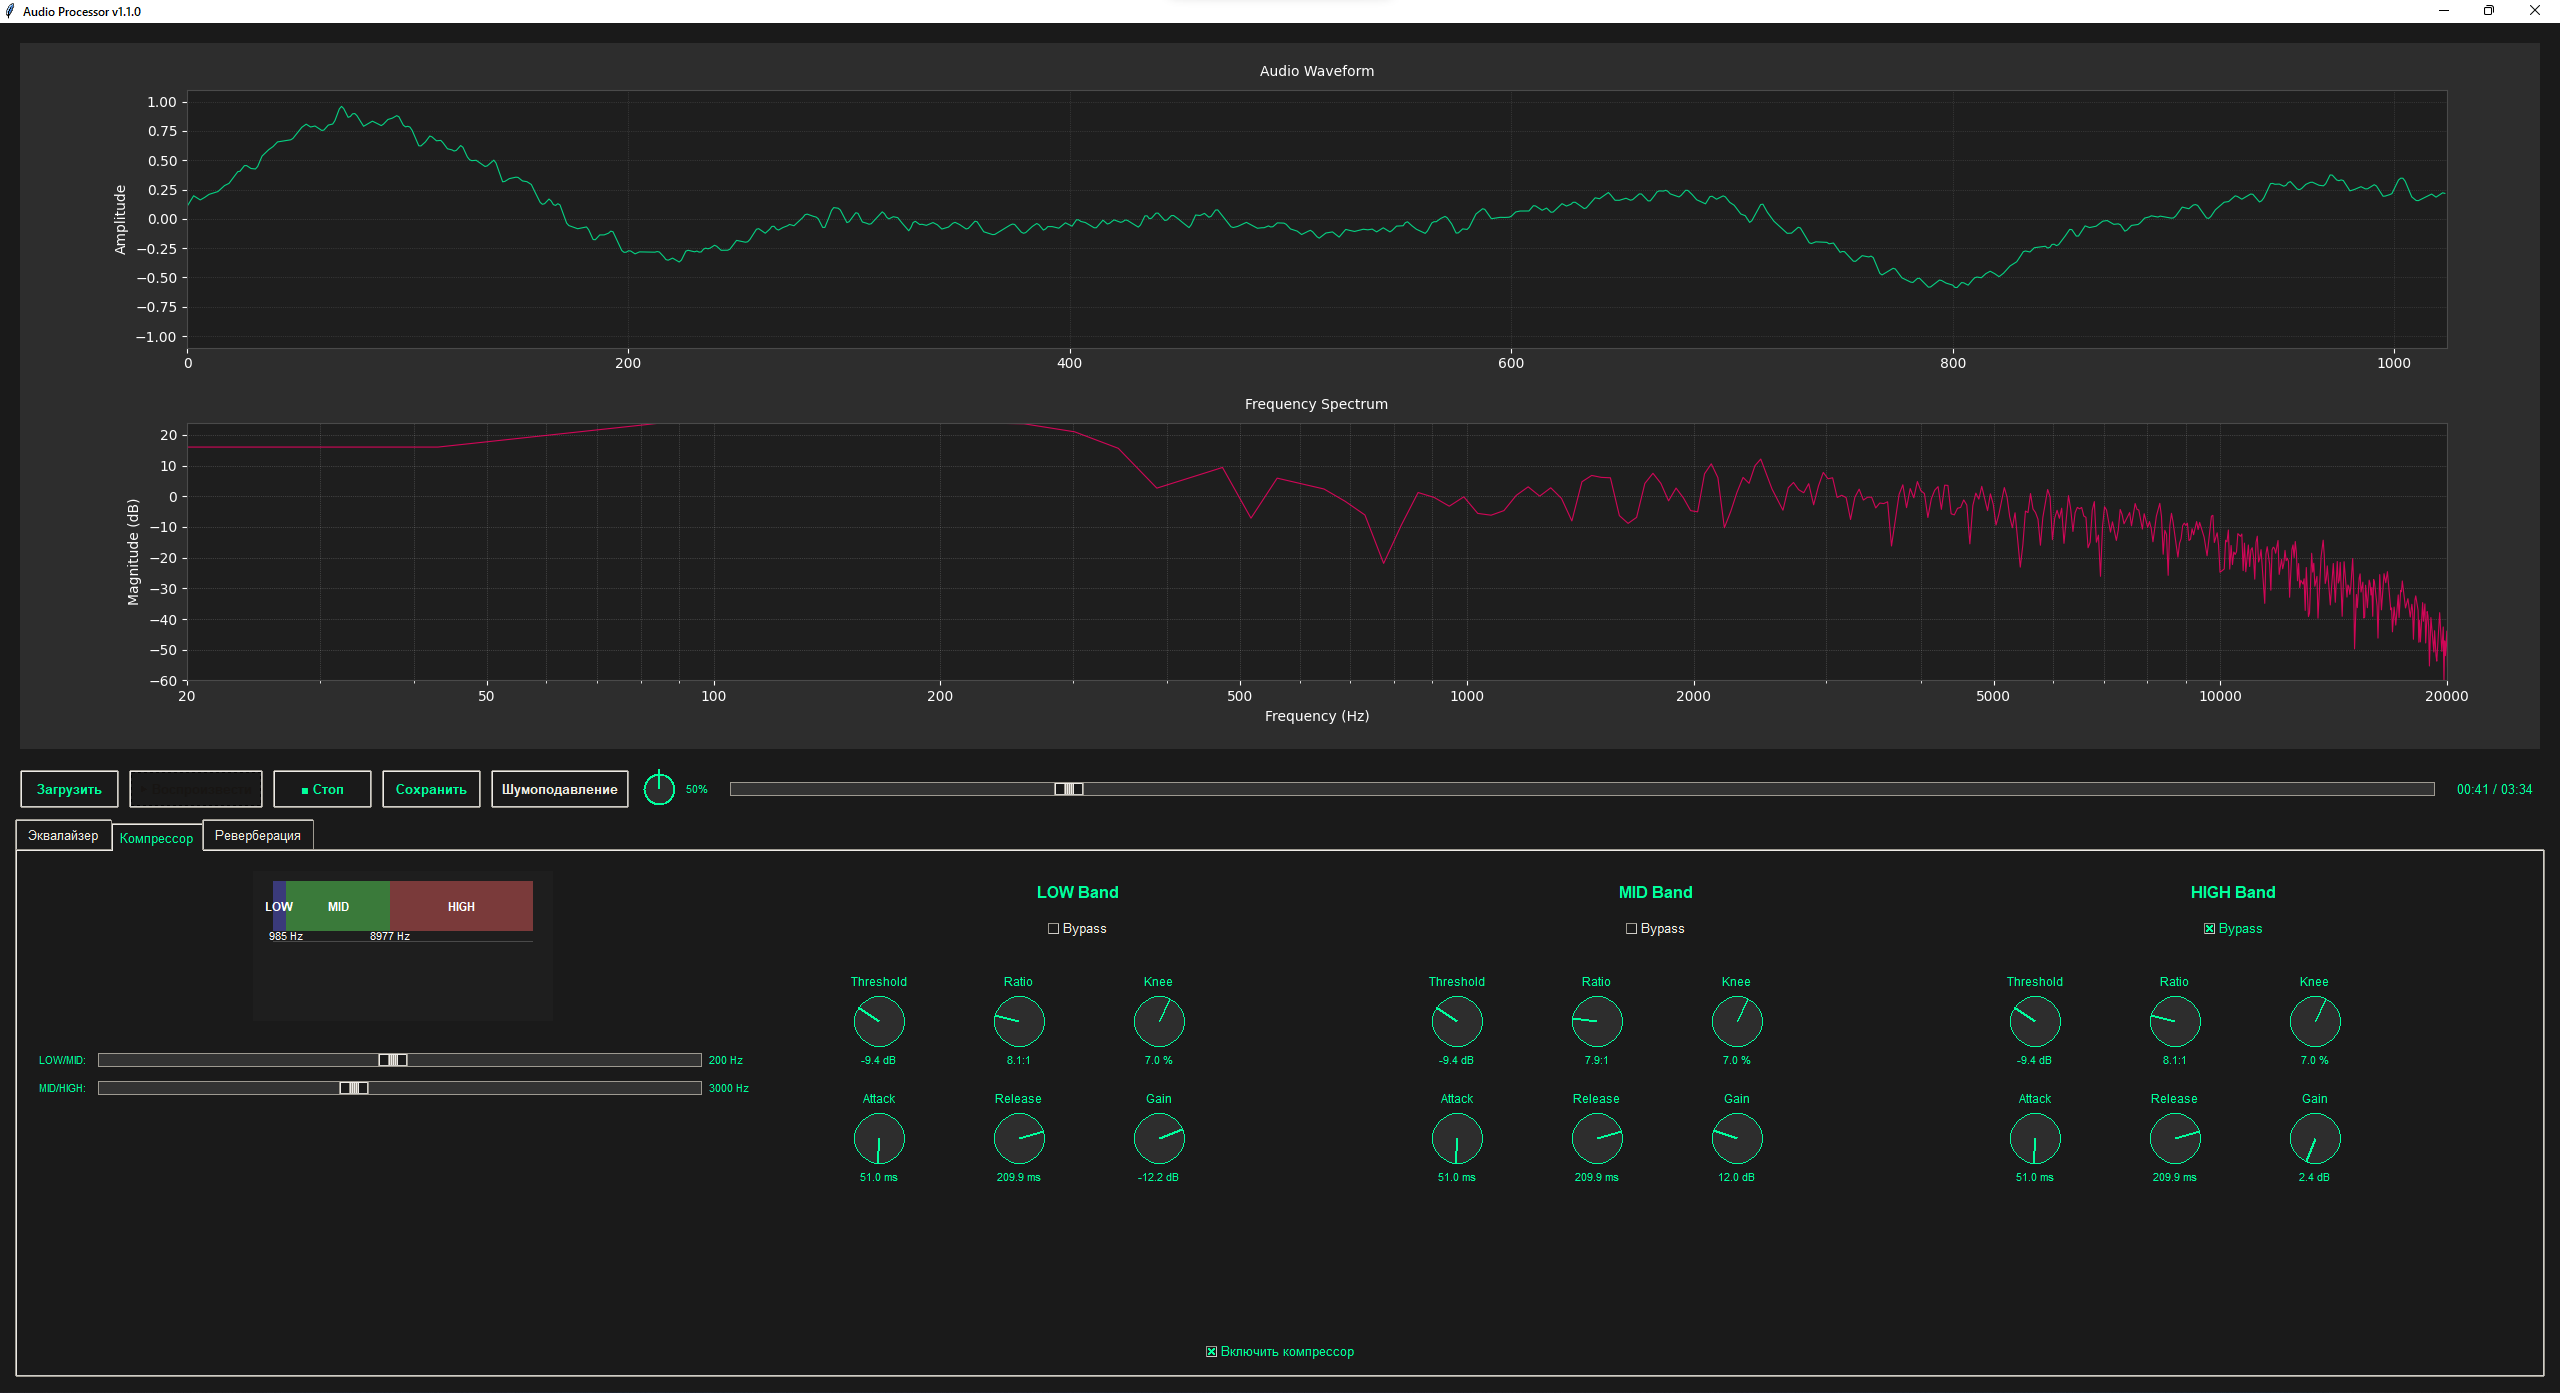
\includegraphics[width=0.8\linewidth]{CompParam}}
	\caption{Изменение параметров компрессора.}
	\label{CompParam:image}
\end{figure}
\clearpage

\textbf{7) Изменение параметров реверберации}

Описание: При изменении параметров реверберации, регулировки knob, все изменения применяются сразу, без задержек и прерываний. Так же изменяются графики формы волны и АЧХ.

На рисунке \ref{ReverbParam:image} изменение параметров компрессора.

\begin{figure}[ht]
	\center{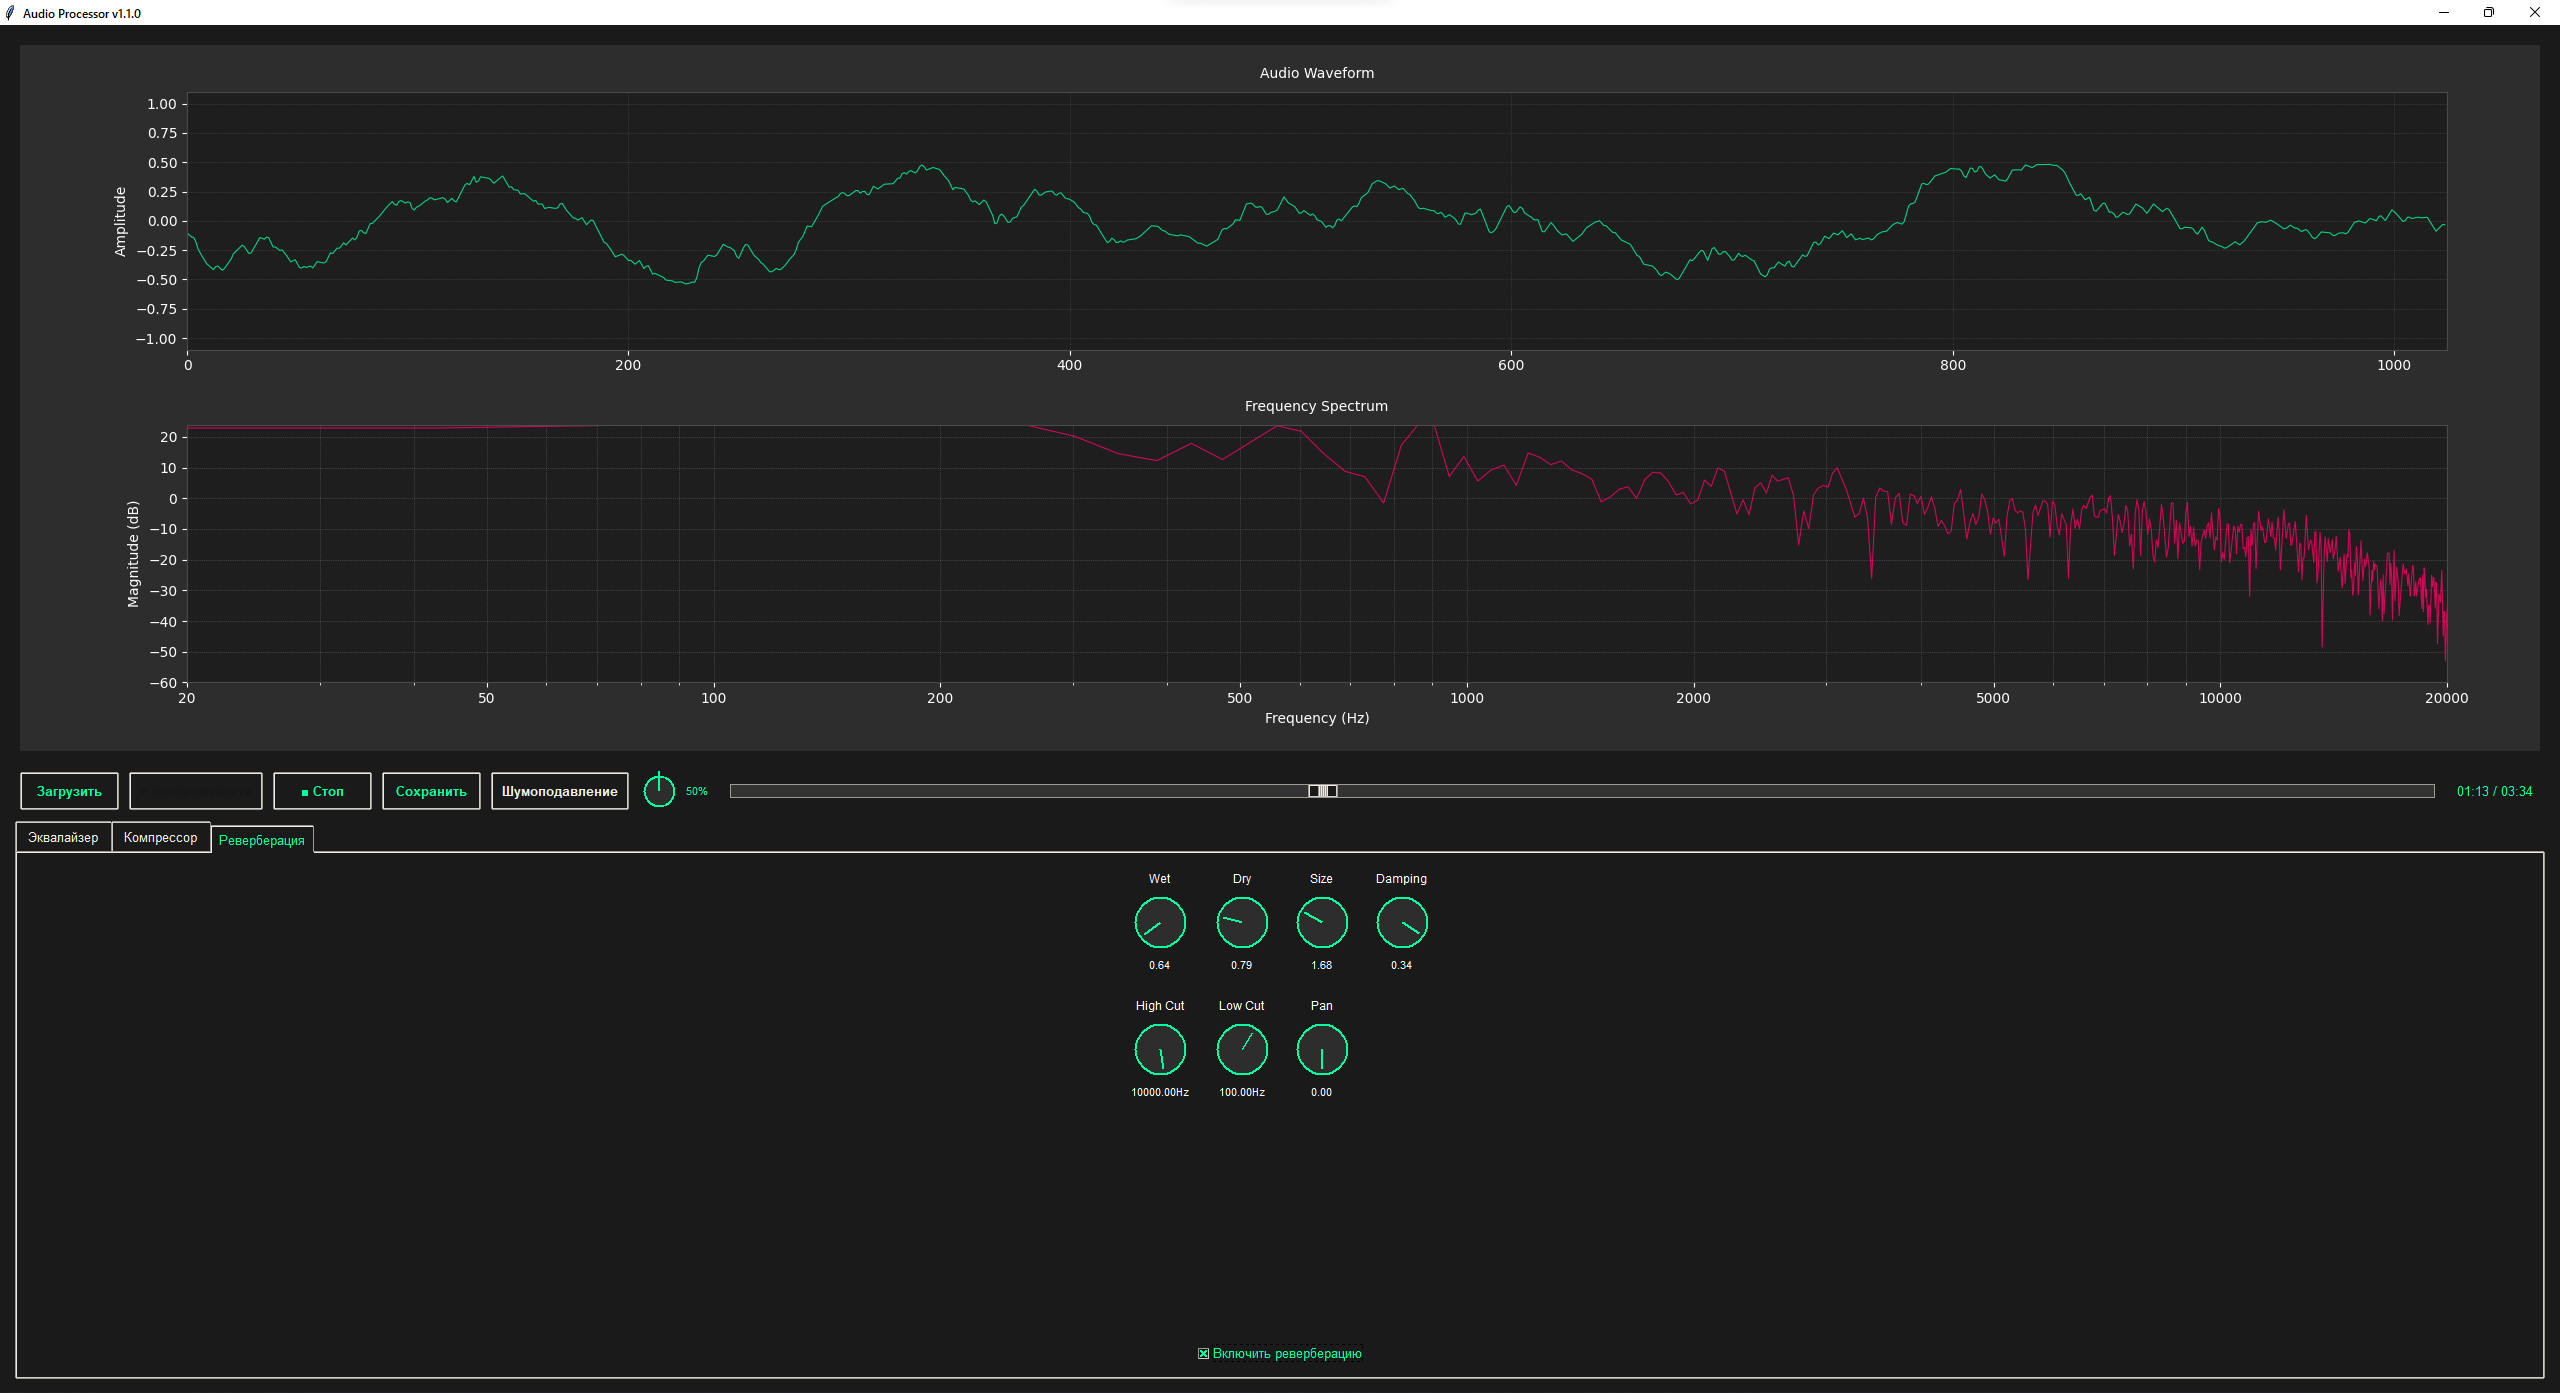
\includegraphics[width=0.8\linewidth]{ReverbParam}}
	\caption{Изменение параметров реверберации.}
	\label{ReverbParam:image}
\end{figure}
\clearpage

